\documentclass{article}
\usepackage{graphicx}
\graphicspath{ {graphs/} }
\usepackage{geometry}
\geometry{a4paper, portrait, margin=1.0in}
\usepackage{gensymb}
\usepackage{booktabs}
\begin{document}
\begin{titlepage}
    \begin{center}
        \vspace*{1cm}
        
        \Huge
        \textbf{Reconstruction of Charge Number of Heavy Cosmic Rays using Cherenkov Light}
        
        \LARGE
        
        \vspace{1cm}
        
        \textbf{Robert Stein}\\
        \textbf{CID 00819615}
        
        \vspace{1cm}
        
\includegraphics[width=0.4\textwidth]{Imperial_College_London_logo} 
        \hspace{0.5cm}
        
\includegraphics[width=0.4\textwidth]{hamburglogo}
        
        \vspace{1cm}
        
        Supervisor: Professor Dieter Horns
        
        \large
        \vspace{1.0cm}
        
        A thesis presented for the degree of\\
        \textbf{Master in Science}
        
        \vspace{0.5cm}

        Physics Department\\
        Imperial College London
        
        \vspace{0.5cm}
        
        \today
        
    \end{center}
\end{titlepage}
\section*{Abstract}
Between impact with the upper atmosphere and decay into a charged particle shower, heavy cosmic ray elements such as Iron emit Cherenkov Light at an angle determined by the Refractive Index of the air and the energy per nucleon. This direct Cherenkov Light forms a characteristic circular light distribution on the Earth's surface with an intensity proportional to the square of the cosmic ray charge. A new method has been developed to reconstruct this charge number, by fitting the received Cherenkov Photons to the characteristic Lateral Photon Distribution. The expected performance for various existing and planned installations will be discussed.

\section*{Zusammenfassung}
Between impact with the upper atmosphere and decay into a charged particle shower, heavy cosmic ray elements such as Iron emit Cherenkov Light at an angle determined by the Refractive Index of the air and the energy per nucleon. This direct Cherenkov Light forms a characteristic circular light distribution on the Earth's surface with an intensity proportional to the square of the cosmic ray charge. A new method has been developed to reconstruct this charge number, by fitting the received Cherenkov Photons to the characteristic Lateral Photon Distribution. The expected performance for various existing and planned installations will be discussed.
\newpage
\tableofcontents
\newpage

\section{Preface}
I basically just did everything. It was great.
\newpage

\section{Introduction}
There are numerous Telescope Arrays which image the Cherenkov Light emitted by Cosmic Rays in the atmosphere, including the HESS, MAGIC and VERITAS Experiments. All rely on Hillas Analysis with extracted parameters from each of the camera images being used to reconstruct the events, but heavy atmospheric blurring means that charge resolution is very poor. For Iron Nucleus events, we would expect to reconstruct \[Z \approx 26 \pm 5 \] with a core position resolution of roughly $d \approx 20 m $ \cite{hess07}. 

Cosmic Rays that are imaged by these telescopes have energies between $13 $TeV and $200 $TeV. At present, no study of the relative abundance of different cosmic ray elemental abundances exists at these energies. It could provide important clues regarding the mechanism of Cosmic Ray formation and propagation in the galaxy, but current charge resolution from Hillas Analysis is not small enough to undertake such a study.

Instead of Hillas Analysis, we consider a new method for event reconstruction, in which we fit the known Direct Cherenkovn (DC) Light observed by each telescope to a characteristic Lateral Photon Distribution (LPD) function. This new technique is valid both for currently running experiments, as well as planned experiments such as the Cherenkov Telescope Array (CTA). It uses only the information from the DC Pixel identified in the shower images.

A theoretical study by Kieda in 2001 \cite{kieda01} suggested that for a core position resolution of $d \approx 5 $ m, we could expect to see a charge resolution of $ \sigma_{Z} \approx 1 $ for elements of $Z = 20$ or higher. In this case the core position resolution would be the limiting value. Thus, if the LPD method can achieve this core position resolution, the precision will be sufficient to extract the abundances of the different Cosmic Ray Elements. This the prime motivation for the new LPD technique.

\section{Cosmic Ray Event Simulation}
In order to reconstruct events using the LPD method, we require saturation of the Cosmic Ray Energy, and that the event can be seen by at least 4 telescopes. These restrictions confine us to Cosmic Rays with specific characteristics.

\subsection{Cherenkov Emission}
Cosmic Rays follow a well-defined power law where $ \frac{dN(E)}{dt} \propto E^{-\gamma} $ and experimentally $ \gamma = 2.7 \pm ? $. Consequently higher energy Cosmic Rays are heavily suppressed. The Energy Threshold for Cherenkov Light Emission as a function of height is illustrated in \ref{fig:generalenergy}. Once the Energy of a Cosmic Ray exceeds the local Cherenkov Energy Threshold of the atmosphere, the Nucleus will begin emitting a ring of Cherenkov Light. 

Above threshold, Cherenkov Emission is determined by the Frank Tamm formula!!!!! A full simulation of the LPD was undertaken. Under the assumption of constant magnetic permittivity and a zenith angle of $90\degree$ we can use the approximate form \[ N_{photons} \approx (37000 \times Z^{2} \times \Delta_{h} \times \Delta_{E})\] where $\Delta_{h}$ is the vertical distance travelled in meters and $\Delta_{E}$ is the emission energy range in eV.

If we divide the number of emitted photons by the area of the annulus between the ring radii at $h$ and $h - \Delta_{h}$, we retrieve the LDF shown in \ref{fig:lpd}, which varies with $ \rho_{DC}  = f(r) \times Z^{2}$ . Thus the amplitude of the LDF is proportional to the charge of the Cosmic Ray, enabling the Charge to be determined from the DC emission. This is the basis for charge reconstruction in the LDF method.

\begin{figure}
\begin{center}
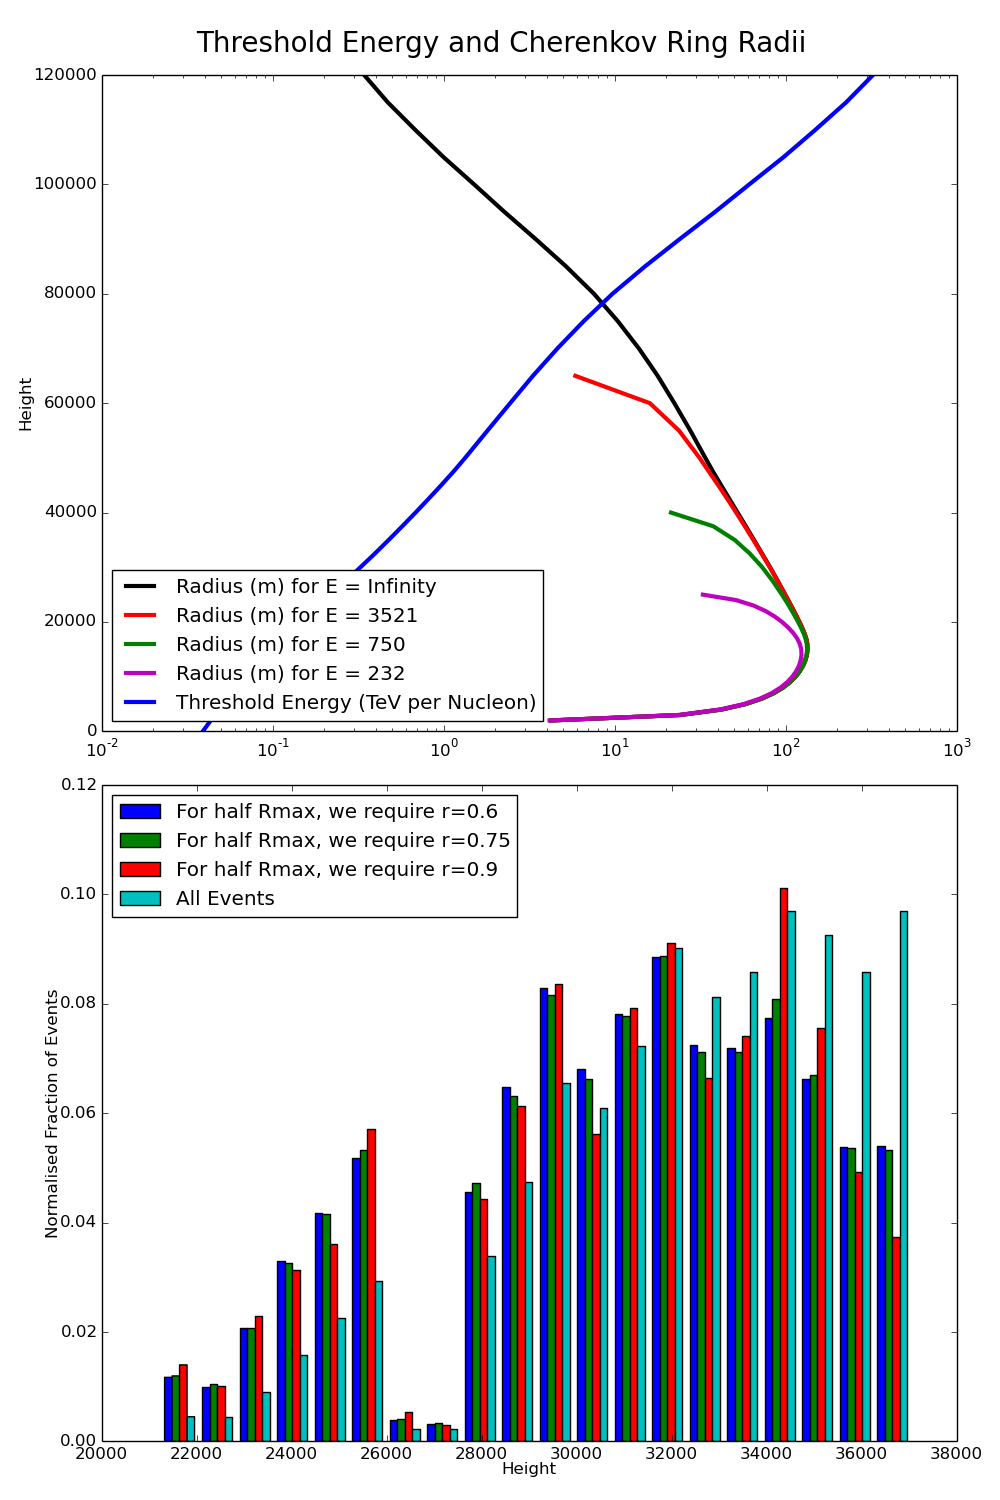
\includegraphics[height=0.9\textheight]{logenergyradius}
\caption{The Threshold Energy for Cherenkov Emission is marked in blue. With the assumption of $\beta=1$, the maximum emission radius is marked in black. The red and green and magenta line show the emission radius at 3.57 and 0.75 and 0.23 TeV per Nucleon respectively. The Green line is sufficiently close to the background to be saturated at 24km, while the magenta line is not.}
\label{fig:generalenergy}
\end{center}
\end{figure}

\begin{figure}
\begin{center}
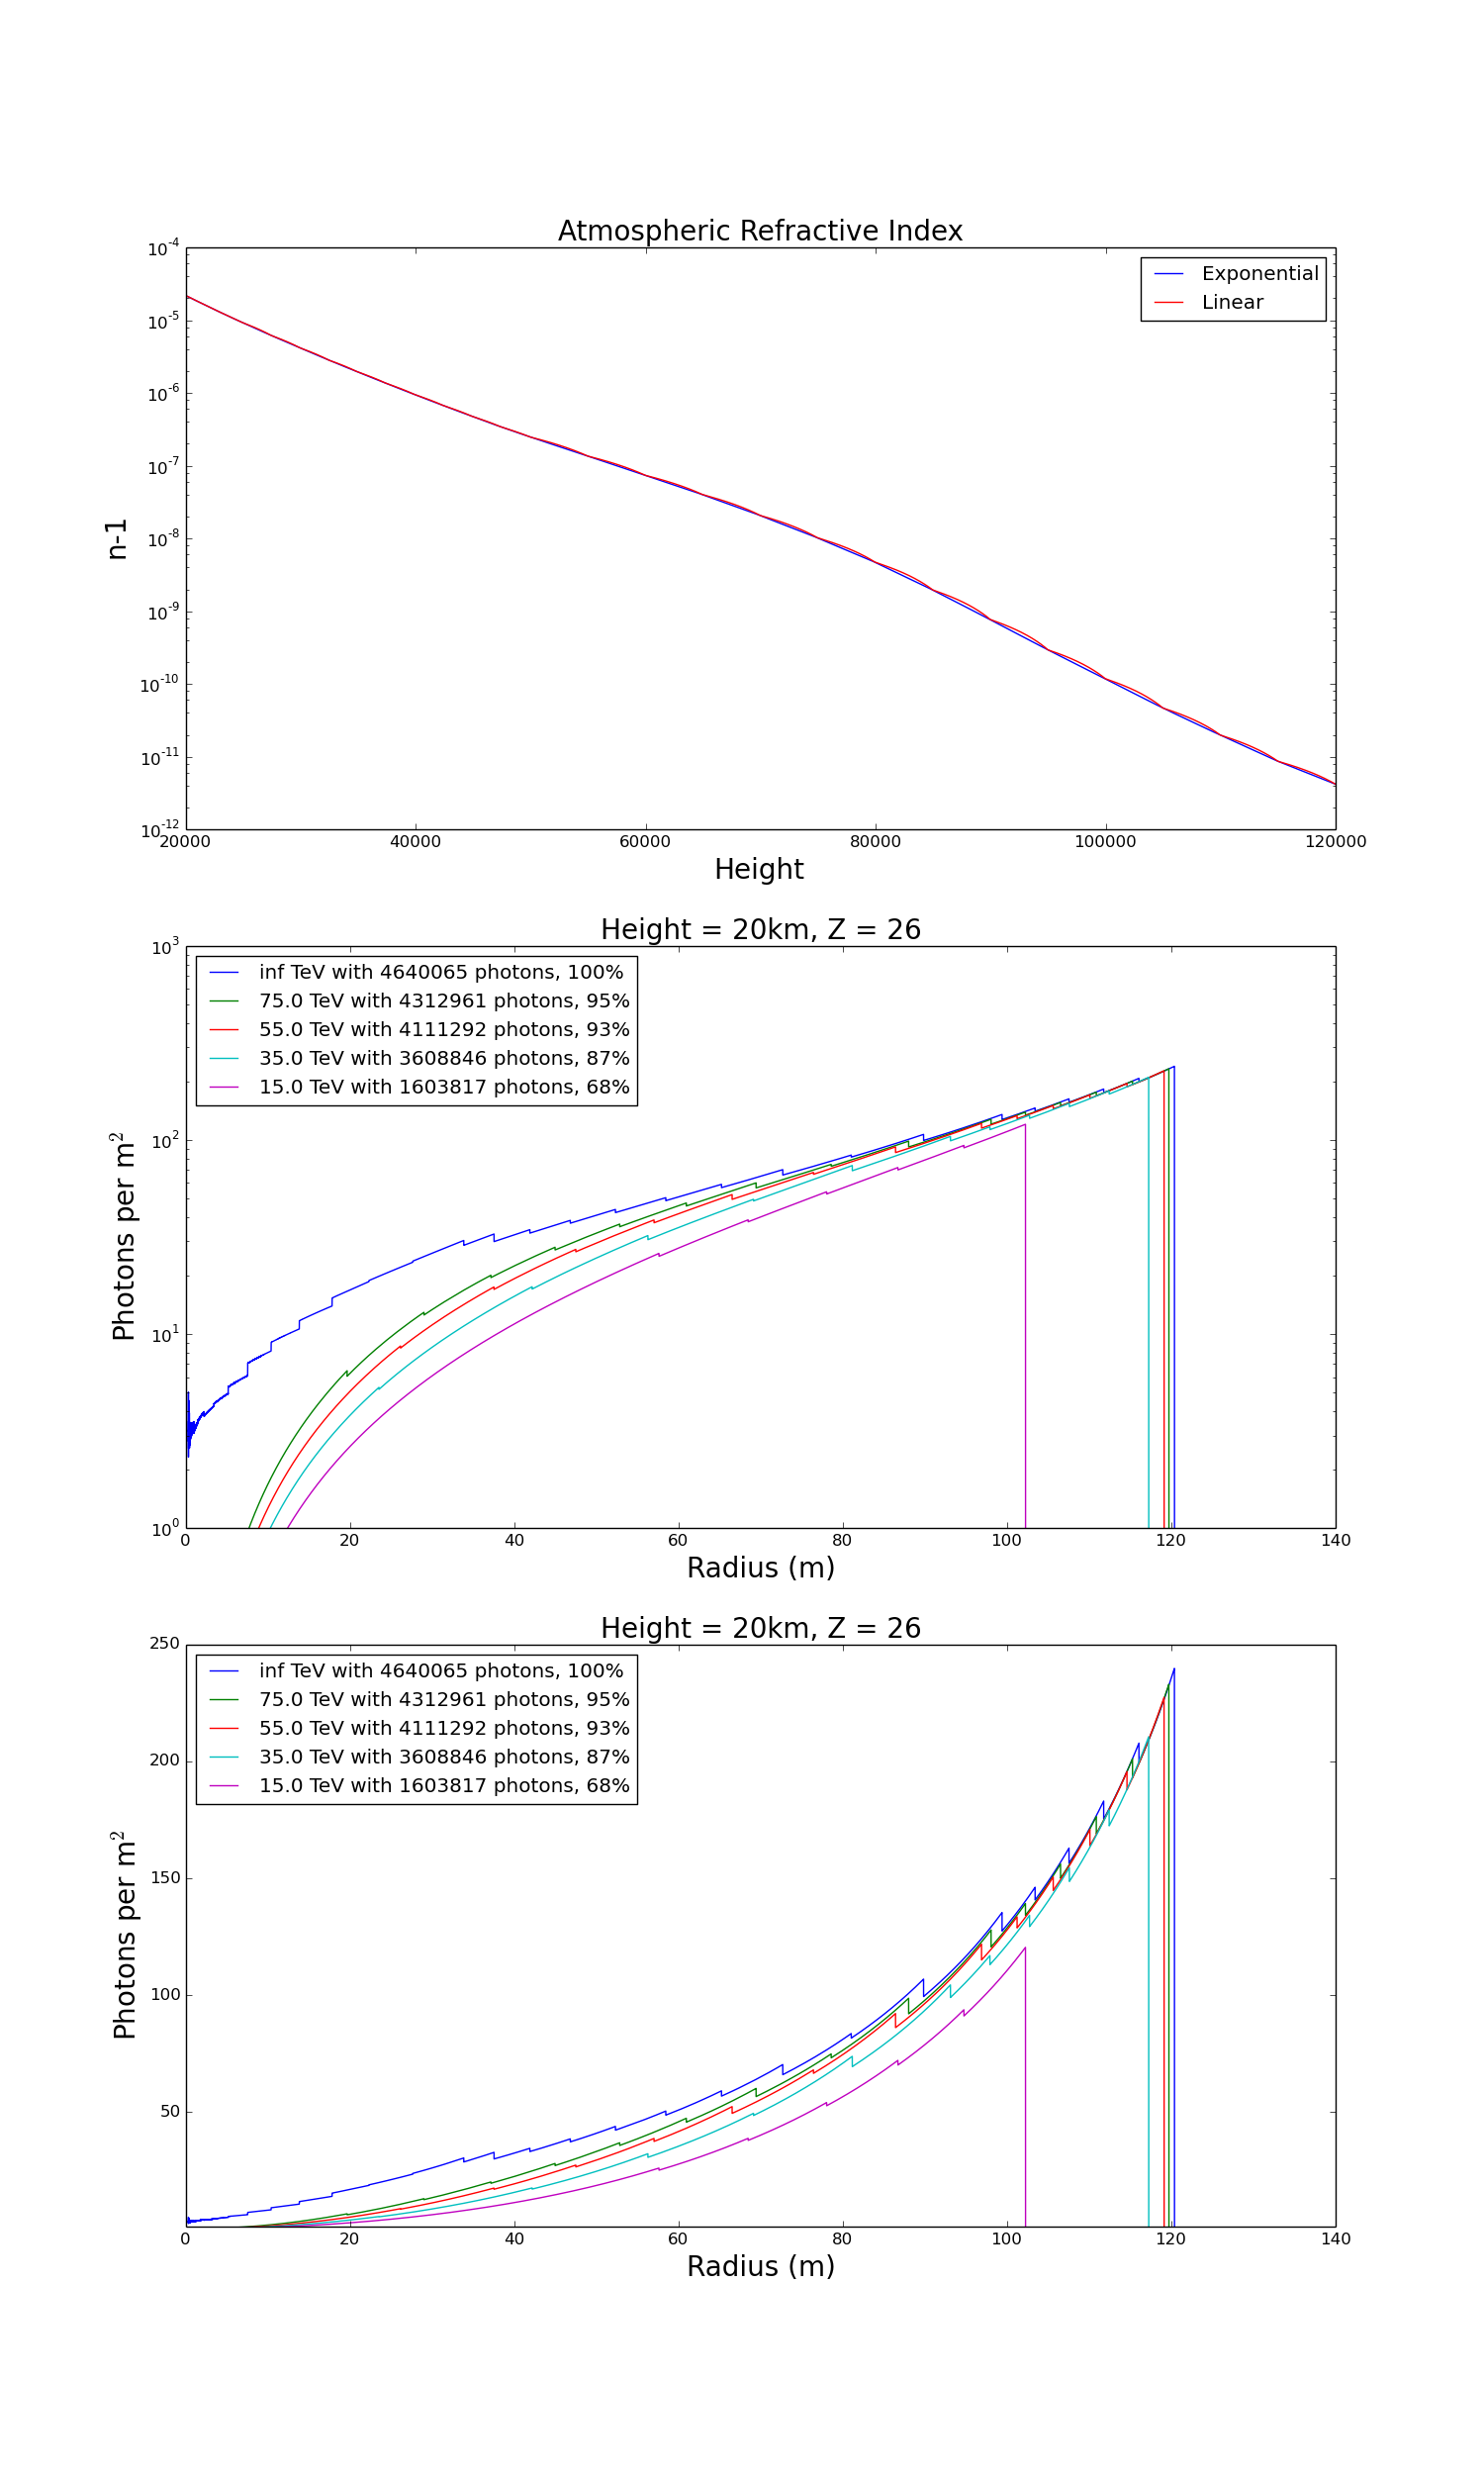
\includegraphics[height=0.9\textheight]{simulatedlpd}
\caption{The LPD obtained from simulation of an Iron Nucleus up to a first interaction height of 25km for a range of Core Energies. An altitude of 1.8km for the experimental array is assumed. Atmospheric absorption, although neglected, is broadly constant across the emission range leading to uniform amplitude scaling.}
\label{fig:lpd}
\end{center}
\end{figure}

The Refractive Index of the atmosphere, and thus the Cherenkov angle $\theta_{C}$, increases as the altitude decreases. The refractive index at a series of heights, based on data from the HESS site, is shown \ref{fig:lpd}. Exponentials are fitted between points to provide interpolation, and a comparison can be made to a linear interpolation that is also plotted. Despite the exponential interpolation, discontinuities in the second derivative of the refractive index prevent the LPD from being smooth in the simulation. This is unimportant, because in reality the variation due to atmospheric conditions and random noise will smear out any discontinuities in the LDF.

Emission continues until the first interaction with the atmosphere, occurring at a randomly distributed height we call $h$. Then for a given Telescope Array altitude above sea level, simple trigonometry yields the radius of the LDF on the ground:
\[ Radius(height = altitude_{array}) = \tan [\theta_{C}(h)] \times (h - altitude_{array})\]

Thus the upper atmosphere emission contributes to the inner LDF, while the lower atmosphere emission contributes to the outer LDF. We can also see ground emission radius as a function of height in \ref{fig:generalenergy}. We find that the high-radius emission (occurring near the first interaction region) varies little between different high energies. We deem this to be \textquoteleft Saturated Emission\textquoteright.

To accurately quantify Saturated Emission, we can compare the photon density to the theoretical maximum photon density, corresponding to an infinite-energy particle with $\beta =1$. The illustrated maximum is useful as a reference, although because the atmosphere is not modelled beyond an altitude of 120km, the small-radius emission is not accurately simulated entirely correctly. However, real cosmic rays in the considered energy regime will all cross the emission threshold and begin emission at an altitude much lower than 120km, so can be considered accurately modelled. Absorption WAS/WAS NOT modelled.

However, in the 4 telescope height region, the Cherenkov Threshold Energy is $ E_{Threshold} \approx 0.35$ TeV per Nucleon as shown in \ref{fig:lpd}! The saturation in for these heights occurs roughly at 0.7 TeV per Nucleon or something...

\subsection{First Interaction Height}
Cosmic Rays survival in from the top of the atmosphere follows an exponential decay with the number of 'interaction lengths' passed. The interaction length is dependent on the interaction cross section, which increases with density. Thus the number of interaction lengths increases exponentially as height decreases. The resultant decays occur most often at a height of $h \approx 40 \pm 10$ km , as seen in \ref{fig:generalheight}.

\begin{figure}
\begin{center}
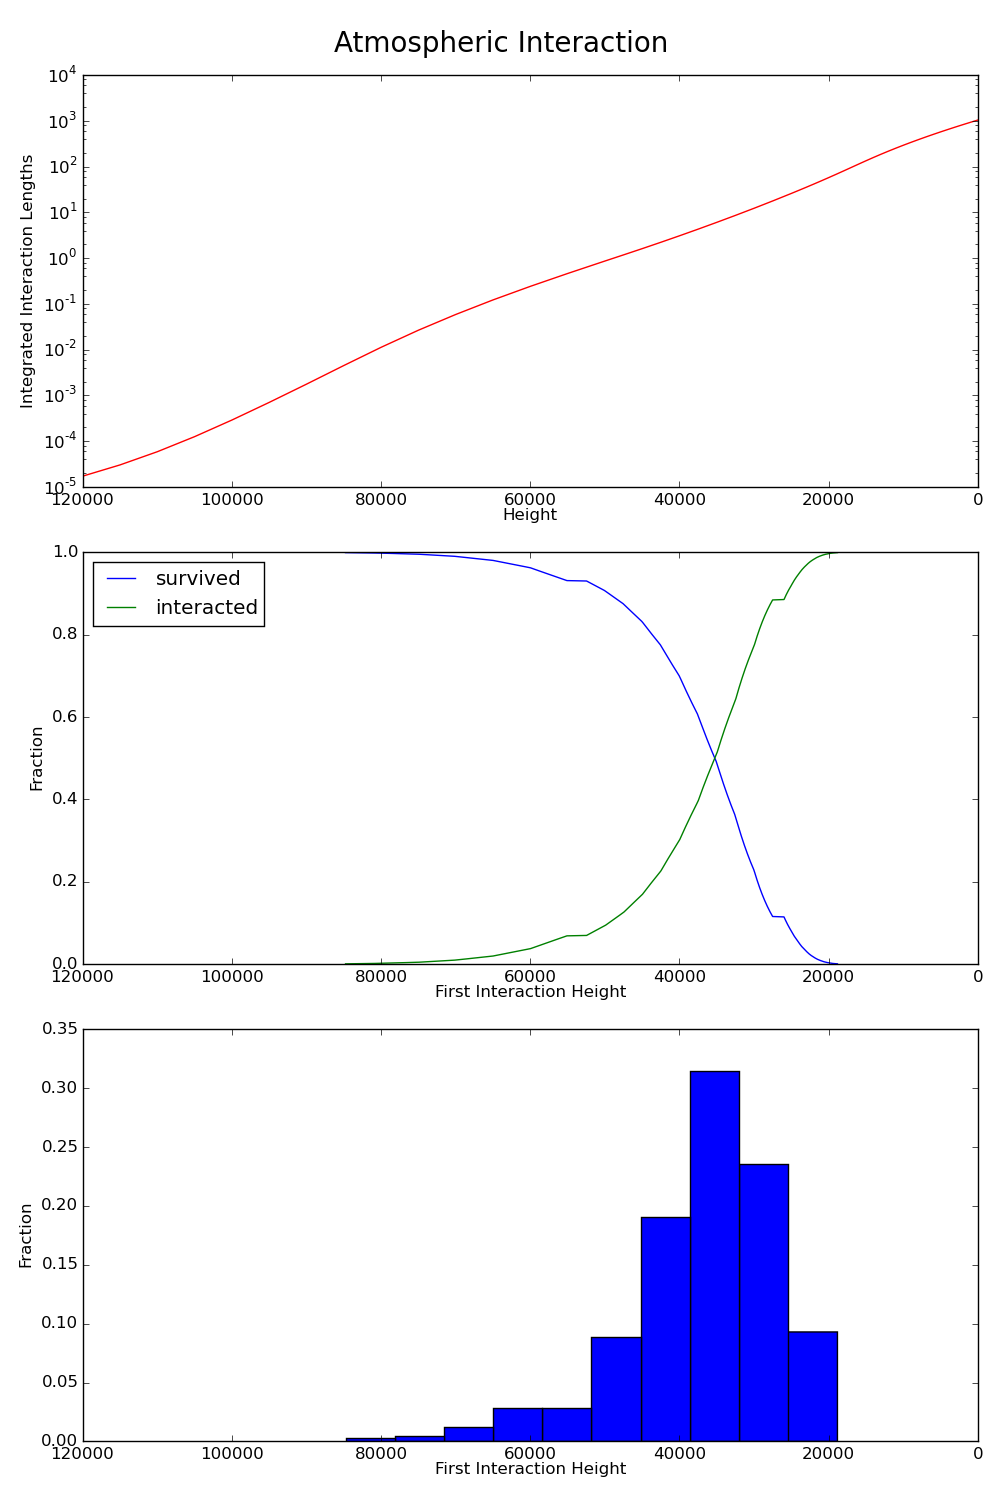
\includegraphics[height=0.9\textheight]{generalheight}
\caption{The integrated interaction lengths increases as height decreases. Thus the decay probability follows a exponentially increasing distribution. The mean first interaction height for all events is roughly 40km above sea level.}
\label{fig:generalheight}
\end{center}
\end{figure}

\subsection{Atmospheric Absorption}
The Cherenkov Light, mostly emitted in the visible blue part of the EM spectrum, experiences relatively little atmospheric absorption. The major of Rayleigh scattering-based atmospheric absorption occurs in the lower part of the troposphere, and thus the atmospheric absorption is almost independent of emission up to first interaction height.

\section{LPD Event Reconstruction}

\subsection{Log Likelihood Minimisation}
In order to fully reconstruct an event, we need to find the x/y core position, the Energy per Nucleon, the first interaction height and the charge. However, if one telescope in a five-telescope array does not observe DC light, this data point can be used to constrain the core position. Thus, for the LDF method to be applied, we require a minimum of five telescopes, four or more of which must image the DC light. We consider the amount of DC light that each telescope receives to be Poissonian \[  P_{i} ( N_{i, Received} \mid X, Y, Z, height, Epn )  =  \frac{ e^{- \lambda_{i} } \times \lambda_{i} ^{N_{i}} }{N_{i}!} \]

In order to reduce computing time, we can use Stirling's Approximation $\ln( N! )  \approx  N \ln(N) - N + \frac{1}{2} \ln(2 \pi N)$. Pure night sky background requires that there be more that X photons in a DC pixel, and for this Stirling's Approximation has an error of just Y?. We then minimise the Log Likelihood function \[ - \ln(L) = - \sum_{i=1}^{n} \ln(P_{i}) \approx  \sum_{i=1}^{n} [\lambda _{i} - N_{i} \ln(\lambda _{i}) + N_{i} \ln(N_{i}) - N_{i} + \frac{1}{2} \ln(2 \pi N_{i})]  \] where n is the total number of telescopes in the array.

\subsection{Extracting Charge Resolution}
Having reconstructed many events, we can then derive the $\sigma_{Z}$ of the dataset, giving us a number to directly compare the quality of event reconstruction. However, a simple Gaussian 68\% method will yield only half integer values of $\sigma_{Z}$ and very frequently 0. This will be unhelpful for comparisons of minor modifications of reconstruction methods.

Instead, we can assume a Gaussian with tails at the highest and lowest reconstructed charge values in the dataset. The size of the dataset can be used to calculate the fraction of events that the extreme values represent, and this probability can be converted into a \textquoteleft number of standard deviations from mean'. Dividing the Gaussian total width by the number of standard deviations gives us a value for $\sigma$. Although this will in most cases tend to overestimate the spread of the data, it will also be sensitive to all increases in the proportion of correctly reconstructed events.

\subsection{Iterative Scanning Minimisation}
Through $\sigma_{Z}$ calculation, we find that the LDF method initially provides very poor charge reconstruction. This is as a result of varying Threshold Energies and the sharp drop in the LDF above the maximum radius, which means the Log Likelihood is frequently discontinuous within the parameter space. Consequently, a Minuit-type minimisation algorithm will only be able to find a local minimum near the starting values for the fit parameters.

To overcome this problem, we can iterate over a series of starting values for the parameters, with the aim of scanning the true minimum among the many minima found. To simplify matters, we can scan only the integer Z values over the range $ 20 \leq Z \leq 32 $, rather than considering the charge to be a free floating parameter.

In order to reduce the number of calculations needed, we can consider the core position region derived from camera images, as in Hillas Analysis. Each telescope will have a Gaussian smeared central axis indicating the direction of the core. We overlay the simulated telescope array with a grid of points with grid width 1m. Then we select all points satisfy the condition of lying within the shower axis direction confidence interval for every telescope. The angular width of the confidence interval from the shower axis will be determined by the precision of the telescopes.

Having determined the relevant Height and Energy ranges, we can then consider combinations of Energy and Height for which the Energy is above the Cherenkov Emission Threshold (and is saturated!). This gives us a second set of starting \textquoteleft Coordinates \textquoteright.

The Z value is fixed and the LL function is then minimised with the assigned starting values, with the other four variables allowed to float freely. Minimisation typically scans 13 Z values, 10 core position coordinates, and 50 Height/Energy coordinates, yielding $ 13 \times 10 \times 50 = 6500$ minimisations in total. Such a technique is resource intensive but reduces $\sigma_{Z}$ by a factor of 5 or more. (CHECK this quantitatively and get a graph yo. Want to see some plateauing of sigma Z!).

\subsection{Boosted Decision Trees}
Using one quarter of a large sample of Monte Carlo data, we can train a Boosted Decision Tree (BDT) for a given telescope multiplicity, using the reconstructed x/y core position, height and energy, as well as the Log Likelihood. The BDT is told whether each event is \textquoteleft signal' (correctly reconstructed) or \textquoteleft background' (incorrectly reconstructed). 

For every simulated event, this trained BDT can then be used to assign a \textquoteleft Signal Probability'. On a second quarter of the dataset we can optimise a cut on the minimum signal probability, in order to maximise the ratio of signal to background. We find that the $\sigma_{Z}$ of the remaining \textquoteleft Test' Monte Carlo data is reduced when the same BDT cut is applied.

\section{DC Pixel Identification}
\textbf{Cosmic Rays will emit Direct Cherenkov (DC) light in the upper atmosphere, before generating an Extended Air Shower (EAS) through interaction with the lower atmosphere. }

In telescope images, the DC light is usually concentrated in a single  \textquoteleft DC pixel'. Identifying this pixel is challenging, because the brighter EAS Cherenkov light background often overlaps with the DC pixel. In order to apply the LPD method to data, we must first identify the DC pixel in a shower image, and determine the number of DC photoelectrons present. 

We define the variable $Q_{DC} = \frac{Intensity_{N.N.max}}{Intensity}$ as the ratio of the largest neighbouring pixel intensity to the intensity of a given pixel. In previous experiments, the DC pixel candidate was identified by applying a number of cuts to pixels in an image \cite{hess07}, and from the subset of pixels passing the specified cuts, selecting the pixel with the smallest $Q_{DC}$ as the \textquoteleft DC candidate'. Due to the low pass rate for cuts, we obtain a small low-contamination dataset, while the majority of telescope images are left without a DC pixel candidate. An improved method would aim to increase the number of correctly identified DC pixels, while still enabling cuts which discriminate well between correctly and incorrectly identified DC pixels.

Classifiers provide an alternative method of identification, making use of supervised machine learning to find rules for categorising pixels. To train a classifier, we require a set of training pixels, as well as the correct class for each pixel. Once trained, a classifier can then be used to predict the class of a pixel.

The CORSIKA package \cite{Heck98} was used to generate Cosmic Ray events, and the Sim\textunderscore telarray package  \cite{Bernlohr08} was used to generate corresponding HESS array telescope images.  Simulation with EAS background was used to produce training pixel sets, while corresponding simulation without EAS background was used to find the true DC pixel in each training image. As part of a new method developed for this analysis, a Boosted Decision Tree (BDT) classifier was trained with the data to identify DC pixels. Once trained, the BDT was applied to a separate \textquoteleft testing' set of simulated telescope images. As before, the true DC pixel was determined from a second EAS-free simulation. Thus, the accuracy of BDT identification for test telescope images was calculated.

\subsection{Image Simulation}
The full simulation of air showers was performed using the CORSIKA package, with a standard atmospheric profile derived from measurements conducted at the HESS site in Namibia. In total, 2000 training events and a further 2000 testing events were simulated. The simulated particles were $Fe^{56}$, within the Energy Range of $35-135$ TeV and a spectrum $\phi(E) \propto E^{-2.7}$. For each set of simulated event, 4 unique random number seeds were used to generate the shower. An altitude of 1800m was assumed, again corresponding to the HESS site. The simulated zenith angle ranged from $0\degree < \theta < 2 \degree$, while the simulated azimuth angle ranges from $-2\degree < \phi < 2 \degree$. The four smaller HESS-phase-1 telescopes were arranged in a cross along the x/y axis with the larger HESS-phase-2 \textquoteleft CT5' telescope placed at the center. The length of each cross arm was $85m$. The simulated target region of the cores was chosen to be a square centered on CT5, with each 300m-long side bisecting the x/y axis. 

\textbf{Due to hardware differences between CT5 and the original HESS 1 telescopes, only images from HESS-phase-1 were considered.}

To determine the true class of each pixel, a simulation was initially run with an energy cut of 10 PeV on all muons and electrons. Because this cut exceeded the primary particle energy, neither daughter muons and electrons, nor the photons they would have emitted, were simulated. Thus the hadronic Cherenkov Light from the primary particle and daughter fragments, but not the EAS light, was present in the camera image. A second identical \textquoteleft EAS Simulation' was run including the same random seeds, but without the energy cut on muons and electrons. This gave a complete EAS image including identical DC light.

With the sim\textunderscore telarray package, the expected HESS hardware response to each air shower was simulated. Among other things, the program accounts for atmospheric transmission and density, mirror positions, sizes and reflectivities, camera shadowing and triggering, quantum efficiency and pulse responses. For the full-shower image, the night sky background was also simulated by sim\textunderscore telarray. Due to the comprehensive and detailed nature of these hardware simulations, the resultant images can be considered \textquoteleft realistic'.  However, sim\textunderscore telarray introduces various sources of random noise to the simulation, leading to some divergence in the DC light between the EAS-free and full-shower images.

\begin{figure}
\newgeometry{a4paper, portrait, margin=1.0in}
\centering
\begin{minipage}{0.45\textwidth}
\centering
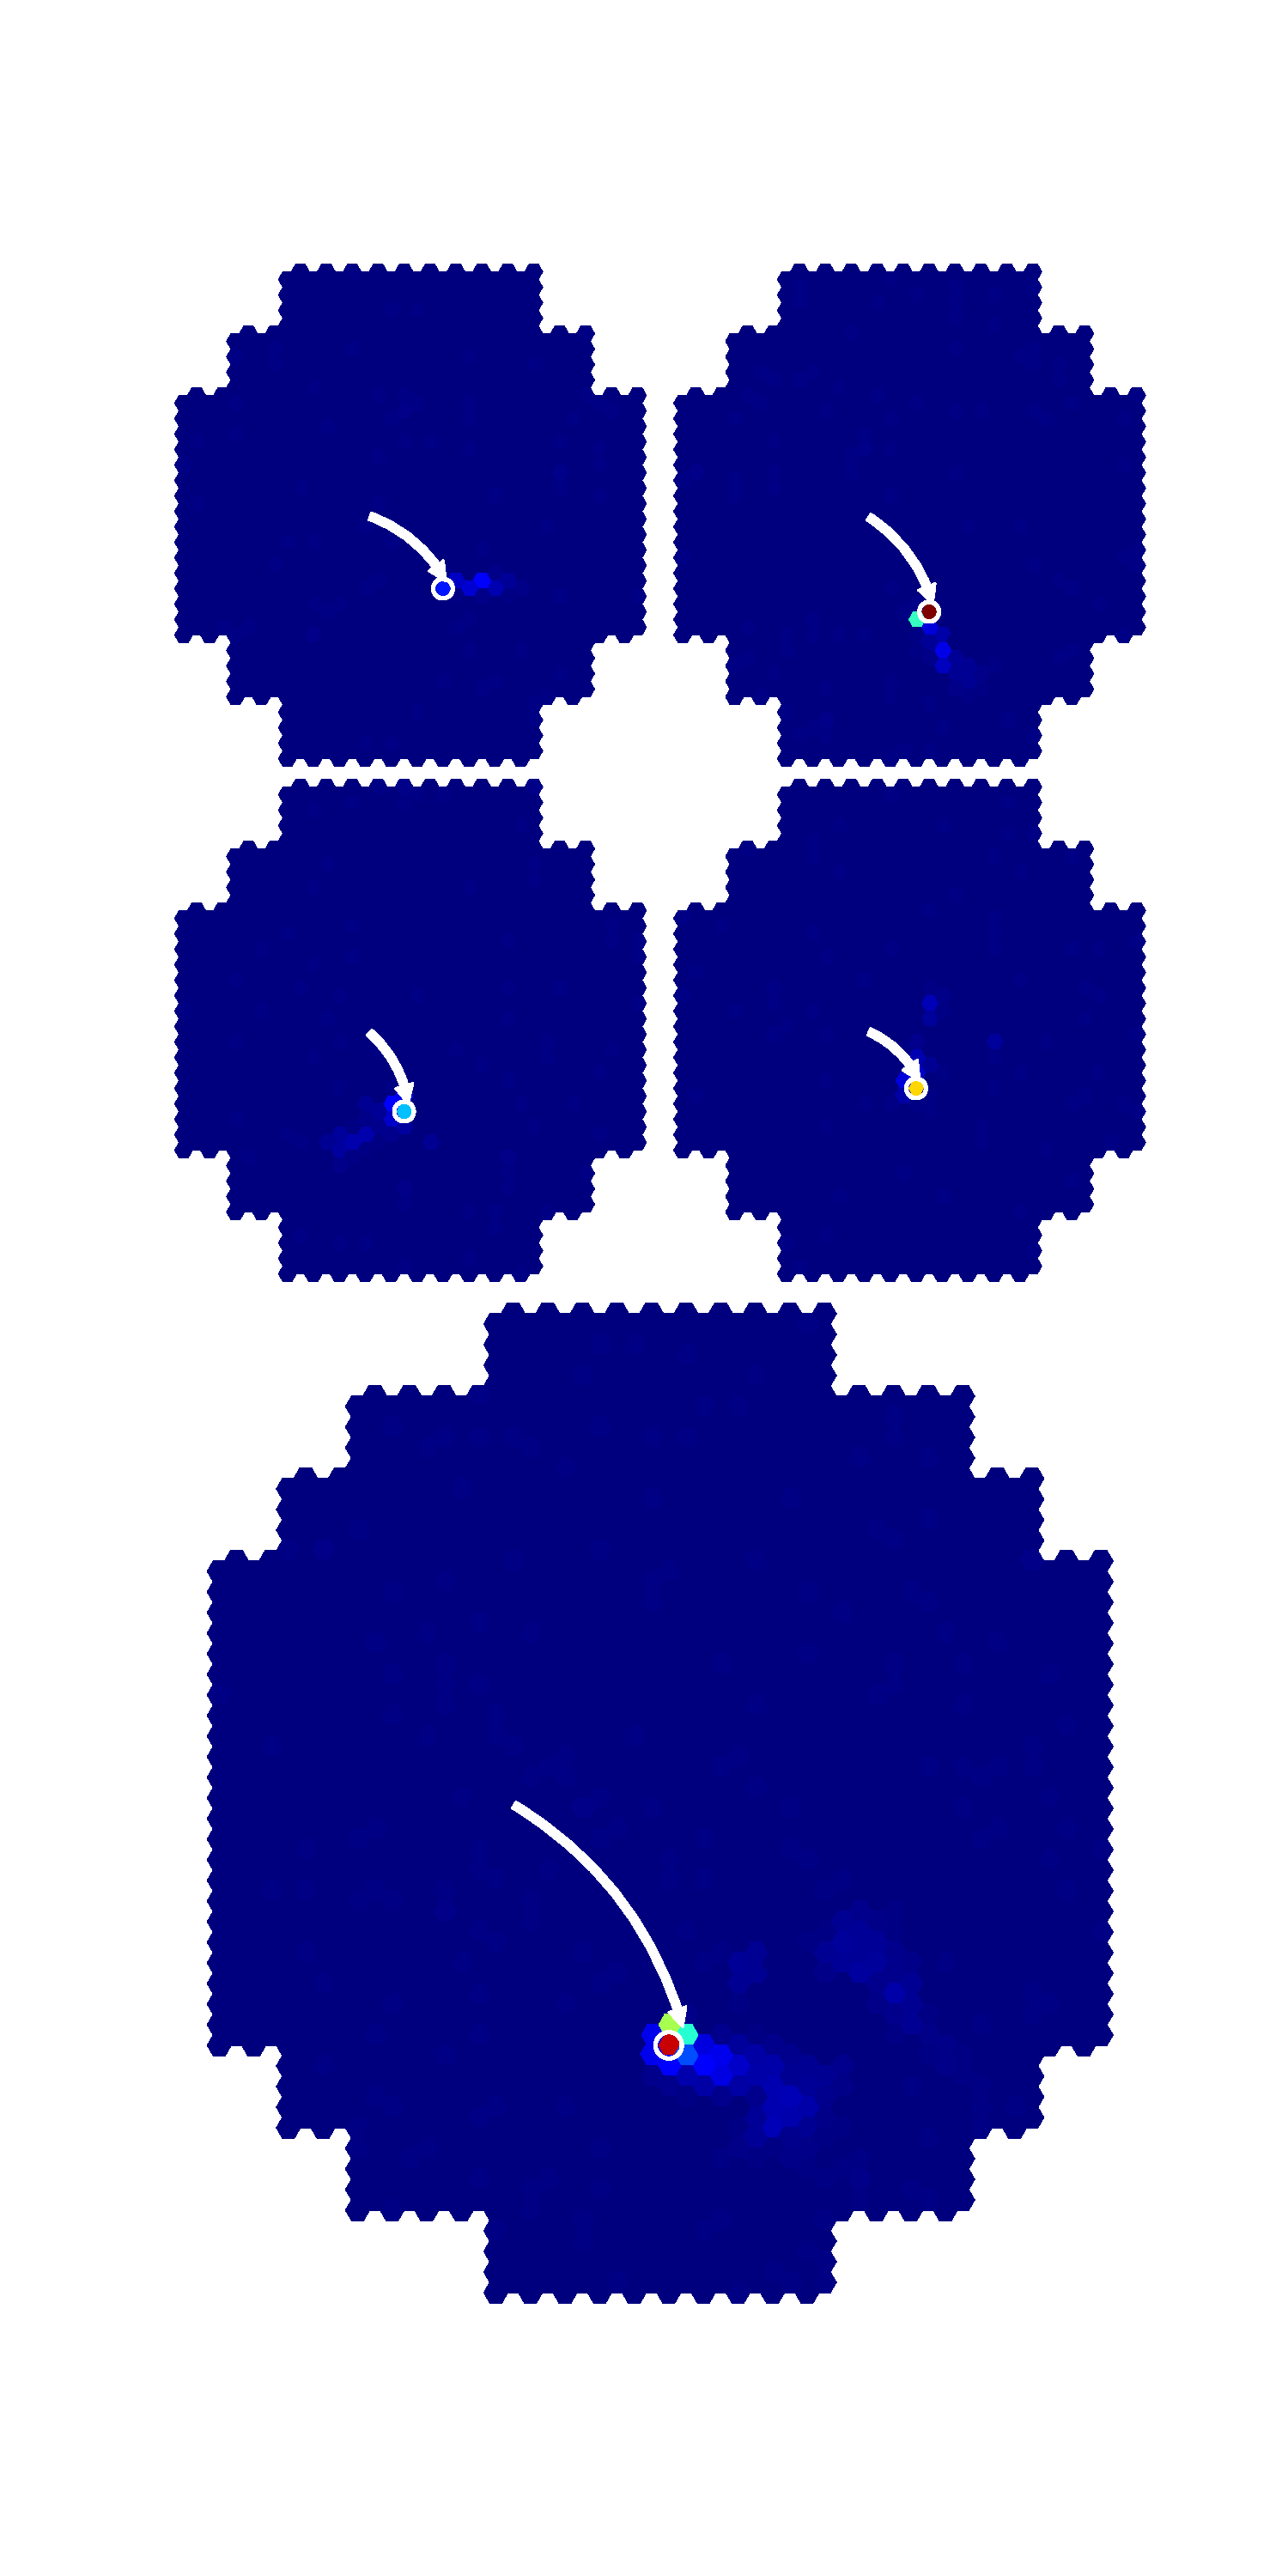
\includegraphics[trim=80 120 80 150,clip,width=\textwidth]{graphDC}
\caption{A typical camera image without the EAS shower. The DC light is visible in every telescope, indicated by the white arrow. The DC pixel is circled in white. The largest telescope image is from CT5, but was not used in analysis.}
\label{fig:DCtelimage}
\end{minipage}\hfill
\begin{minipage}{0.45\textwidth}
\centering
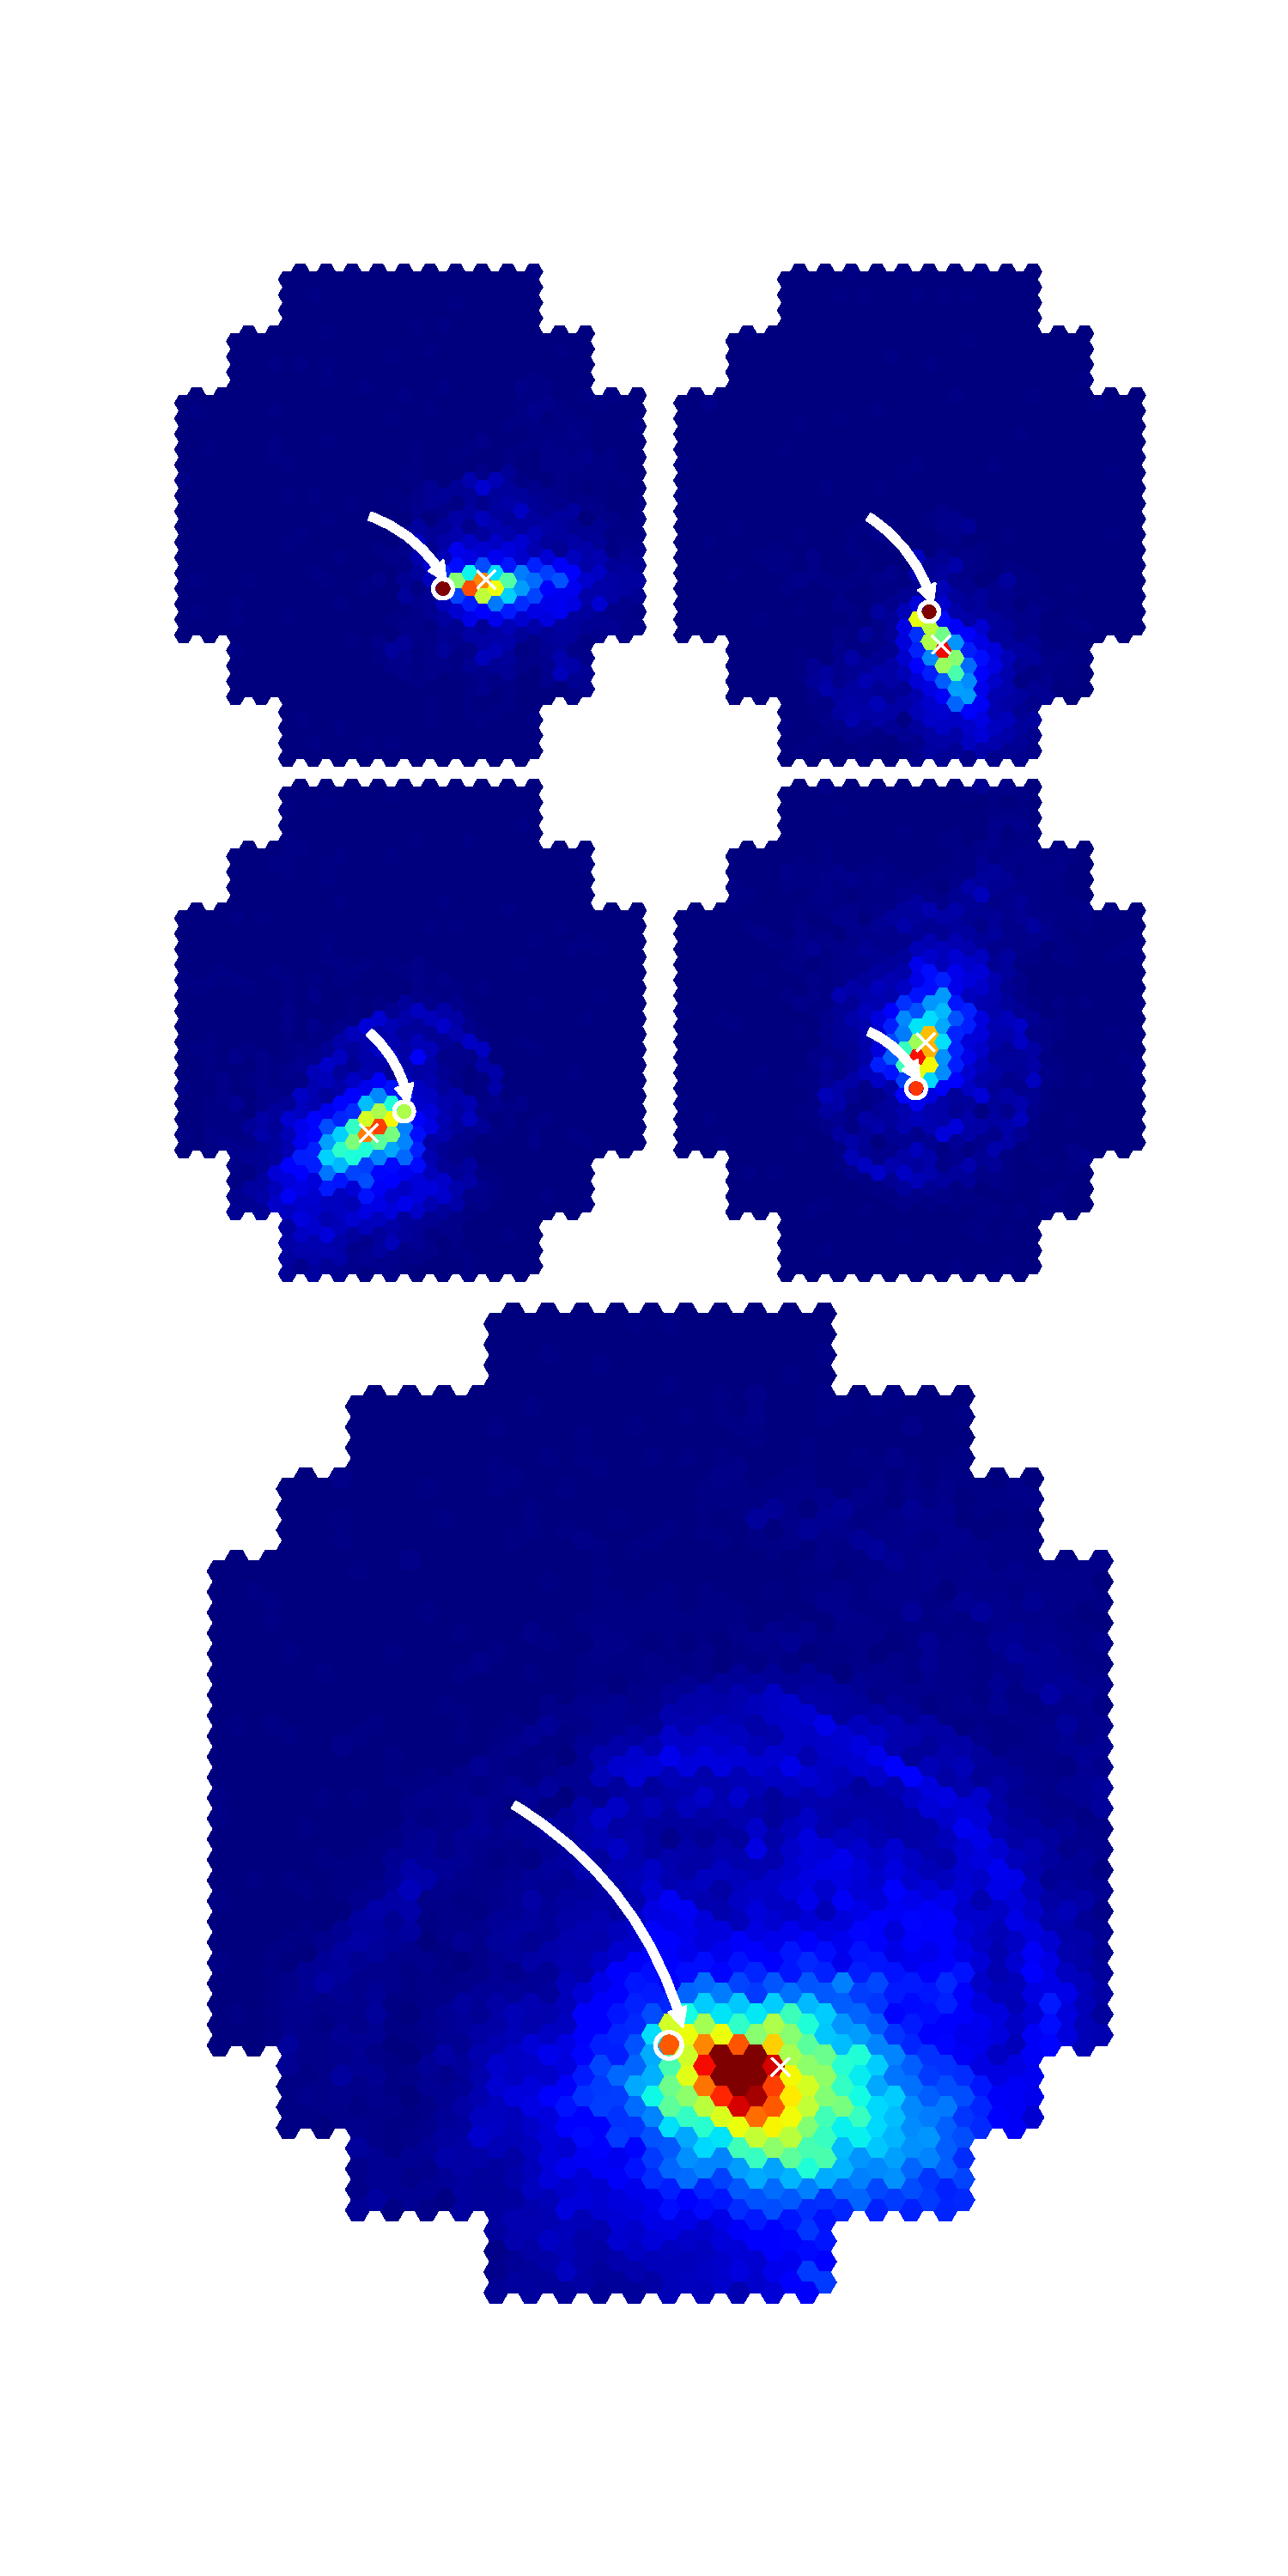
\includegraphics[trim=80 120 80 150,clip,width=\textwidth]{graphfull}
\caption{The same shower as in \ref{fig:DCtelimage} is shown here with the inclusion of the EAS shower. The DC light is pixels indicated with a white arrow and circle. The shower center of gravity is marked by a white cross.}
\label{fig:cutdistribution2}
\end{minipage}
\restoregeometry
\end{figure}

The various pixel entry variables were found from the sim\textunderscore telarray output. The HESS telescope pixels have a high gain Channel 0 and a low gain Channel 1, with both voltages undergoing a Flash Analogue-to-Digital Conversion (FADC). The simulated value of the FADC Voltage for each channel was found. Using the pedestal and gain, the quantity $Intensity = (FADC - Pedestal)\times Gain $ was calculated for each channel. Due to possible saturation of the high gain FADC, only the low gain $Intensity$ was used. Sim\textunderscore telarray also derives various Hillas whole-image parameters. These include the image width and length measured in degrees, from which the aspect ratio $A.R = \frac{width}{length}$ was calculated. The reconstructed shower direction and the shower center of gravity were also calculated, as positions in azimuth and zenith. Additionally the estimated energy and distance from each telescope to core, $r_{core}$,  were found.

For every pixel, in addition to the $Intensity$, its location within the telescope image was determined using the standard HESS layout. The variables $ \Delta_{C.o.G}$, $\Delta_{Direction}$ and $\Delta_{Line}$ were defined as the distance from the pixel to the shower center of gravity, shower direction, and the line joining those two points. Furthermore, the nearest neigbouring pixel IDs were calculated for every pixel position, enabling the $Intensity$ in each neighbouring pixel to be found. The largest neighbouring intensity was identified, and the ratio $Q_{DC} = \frac{Intensity_{N.N.max}}{Intensity}$ was derived. Similarly the largest neighbouring FADC was found, and the ratio $raw_{Q} = \frac{FADC_{N.N.max}}{FADC}$ was calculated. In addition, the Nearest Neighbour Mean Intensity $Mean_{N.N}$ was recorded. The variable $DC_{Signal} = Intensity-Mean_{N.N}$ was defined as an rough guess of the \textquoteleft DC signal' component in the pixel. Lastly the Image Amplitude $I_{tot}$, defined as the total image intensity after the default tail cuts have been applied to the image.

\subsection{Classic DC Pixel Identification}
As a basis for comparison, the original HESS cuts listed in \ref{tab:table1} were replicated for the set of test data. For every image, the total image amplitude $I_{tot}$ was used alongside the zenith angle $\theta$ to determine a dynamic cut, $Q_{DC} < 0.14 \times \log(\frac{I_{tot}}{161 \times \cos \theta})$. Among those pixels passing all cuts, the one with the smallest $Q_{DC}$ was selected as the DC pixel candidate for the image. Because many images had no pixel that passed all cuts, the $Q_{DC}$ method was frequently unable to identify a DC pixel. In the original analysis, an additional cut $r_{core} \textgreater 40m$ was applied. However, the uncertainty in determining the core position through Hillas Analysis is typically of the order of $\pm 30m$. Consequently, this particular cut was omitted.

\begin{table}[h!]
  \centering
  \caption{Cuts applied to image pixel sets, used by HESS collaboration \cite{hess07}}
  \label{tab:table1}
  \begin{tabular}{ccc}
    \toprule
    Variable & Cut\\
    \midrule
     $ \Delta_{C.o.G}$ & \textgreater 0.17 \\
     $ \Delta_{C.o.G}$ & \textless 0.91 \\
     $\Delta_{Direction}$ & \textless 0.45 \\
     $\Delta_{Line}$ & \textless 0.23 \\
     Aspect Ratio & \textless 0.75 \\
     $Q_{DC}$ & \textless 0.14$ \times \log(\frac{I_{tot}}{161 \times \cos \theta})$ \\
    \bottomrule
  \end{tabular}
\end{table}

The candidates were checked against the true DC pixels identified in the EAS-free images. From the testing sample, 5.2\% of all images were correctly identified and passed the cuts. Once misidentified events were considered, the post-cuts sample was 86.2\% accurate, as shown in \ref{fig:cutdistribution}. These values served as a benchmark for BDT performance.

\begin{figure}
\begin{center}
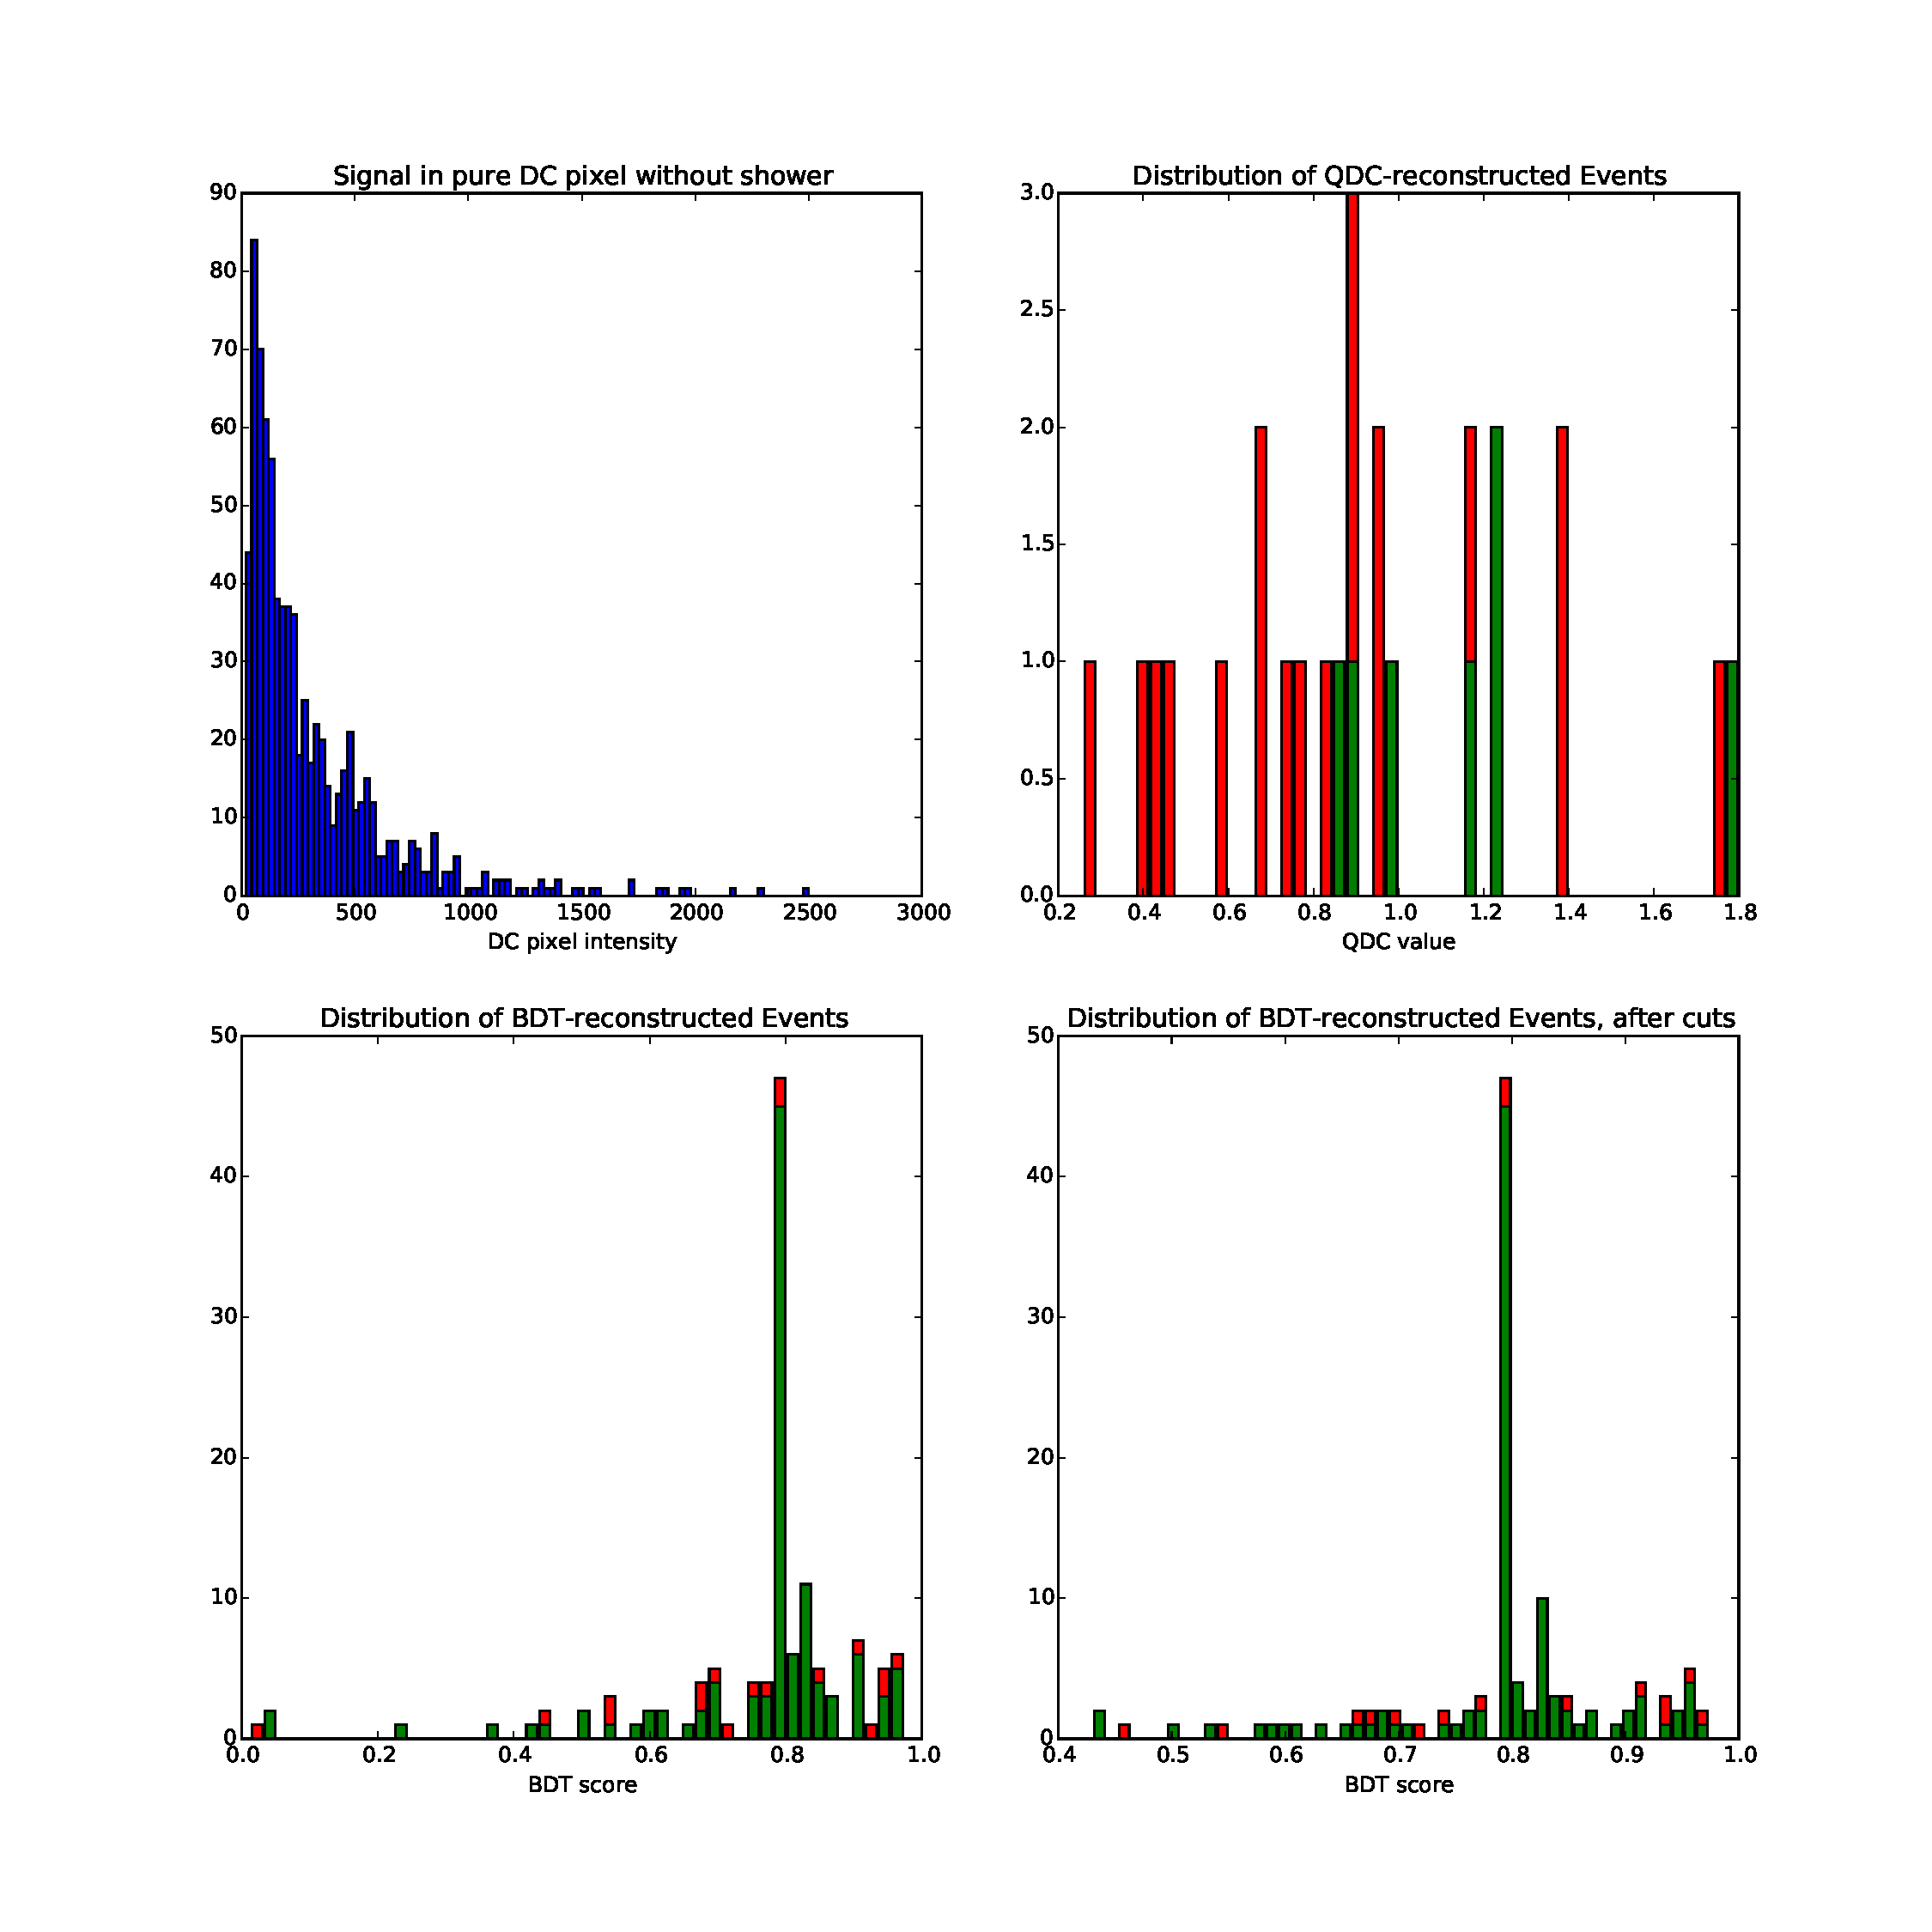
\includegraphics[width=\textwidth]{cutdistribution1None}
\caption{The DC signal in the shower-free pixel is shown in the top left, with a broad gaussian distribution with the tail of the night-sky background extending up to appproximately 5000. Events below this are unlikely to be identified correctly because the DEC light is too faint. In the top right- the distribution of the dataset is shown, once all the non-$Q_{DC}$ cuts have been applied. In the bottom left, the BDT score distribution is shown before any cuts. On the bottom right, we see the same distribution after both signal and BDT score cuts are applied. All green events are ones in which the DC pixel has been correctly identified, while red events are ones that have been incorrectly identified.}
\label{fig:cutdistribution}
\end{center}
\end{figure}

\subsection{Boosted Decision Tree DC Identification}
As an alternative to use of $Q_{DC}$, a new method of DC pixel identification was developed as part of this analysis by using a BDT trained with the Scikit Learn Python package \cite{scikit-learn}. Using the training set of 2000 CORSIKA events, and randomly split further, with 90\% in a learning subset and 10\% in a subset to check for overtraining. Within the learning subset, every HESS 1 image was used, provided it was triggered in both EAS-free and full-shower simulations. For each of the 4.7 million triggered image pixels, an entry was formed with the variables listed in table \ref{tab:hess1classifier}. A class of 0 was assigned to every non-DC pixel, and a class of 1 was assigned to every DC pixel. Having created a dataset, the BDT was then trained with a maximum depth of 8, and with 100 trees generated. The data was provided in the form of individual pixel entries, rather than as discrete sets for images or events.

\begin{table}[h!]
  \centering
  \caption{Relative Feature Importance in HESS-1 BDT training}
  \label{tab:hess1classifier}
  \begin{tabular}{ccc}
    \toprule
    Variable & Relative Importance\\
    \midrule
    $DC_{Count}$ & 0.34\\
    $Mean_{N.N}$ & 0.26\\
    $\Delta_{Direction}$ & 0.11\\
    Image Amplitude & 0.10\\
    $Q_{DC}$ & 0.10\\
    $raw_{Q}$ & 0.05\\
    $\Delta_{Line}$ & 0.02\\
    $Intensity$ & 0.02\\
    \bottomrule
  \end{tabular}
\end{table}

The relative importance of each \textquoteleft feature' is automatically calculated by the Scikit Learn package, and is also recorded in table \ref{tab:hess1classifier}. The variable $DC_{Count}$ was consistently the most importance variable across many combinations of included variables and BDT training parameters. It was found that, under the conditions listed above, the BDT was 99.94 \% accurate for the learning pixel subset, and 99.93 \%  accurate for the overtraining-check pixel subset. This indicates that the BDT was not significantly overtrained, which would otherwise be manifested by a large divergence in accuracy between learning and overtraining-check data.

Having trained the BDT successfully, it was then applied to the same test dataset as for the classic $Q_{DC}$ identification. In each camera image, the event with the largest BDT score was deemed to be \textquoteleft most signal-like', and thus selected as the DC pixel candidate. A cut was applied, requiring $P_{signal} > 0.5$ for the DC candidate to be accepted. A second cut requiring $DC_{Count} > 150$ removed many incorrectly identified events. Application of this combined cut greatly increases the successful identification rate. From the testing sample, 37.3\% of all images were correctly identified and passed the cuts. The BDT was found to be 87.7\% accurate in identifying DC pixels which passed the cuts. This represents a very significant improvement in pixel identification efficiency, as well as a minor increase in accuracy after cuts. 

For LPD event reconstruction, we require events to have a telescope multiplicity $>3$. If we only consider events in which at least four DC pixels were identified, we can determine the high-multiplicity BDT performance. In this case, the fraction of correctly identified DC pixels falls to 16.8\%, while the fraction of incorrectly identified pixels passing the cuts falls to 1.8\%. The sample purity increases slightly to 90.3\%. The relatively high fraction of passing events, in excess of the random expectation of $0.372^{4}=1.9 \%$, suggests that DC pixel identification between different telescope images is strongly correlated. 

However, out of 1245 triggered events, there were none in which the $Q_{DC}$ method identified four DC pixels. Using poissonian statistics, we can place an upper limit of $<0.24 \%$ on the rate of accepted, high-multiplicity $Q_{DC}$ events. Thus, as well as BDT accuracy slightly improving, the performance gap over the $Q_{DC}$ method is vastly increased for high-multiplicity events. The results are summarised in Table \ref{tab:qdcbdtcomparison1}. The BDT method represents a very significant improvement in DC pixel identification over the previous $Q_{DC}$ method, and corresponds to at least a fifty-fold increase in the number of HESS data events that can be studied using the LPD method. Use of this BDT method is thus assumed throughout the rest of this analysis.

\begin{table}[h!]
  \centering
  \caption{Comparison of $Q_{DC}$ and HESS 1 BDT Performance}
  \label{tab:qdcbdtcomparison1}
  \begin{tabular}{ccc}
    \toprule
    & $Q_{DC}$ & BDT\\
    \midrule
    Pixels Accepted and Correctly Identified (\%) & 5.2 & 37.2\\
   Pixels Accepted and Incorrectly Identified (\%) & 0.8 & 5.2\\
    Sample Purity (\%) & 86.2 & 87.7 \\
    \midrule
    High Multiplicity Pixels Accepted and Correctly Identified (\%) & $<0.24$ & 16.8\\
    High Multiplicity Pixels Accepted and Incorrectly Identified (\%) & $<0.24$ & 1.8\\
    Sample Purity (\%) & / & 90.3\\
    \bottomrule
  \end{tabular}
\end{table}

\subsection{HESS-2 BDT}
The original HESS study predated the construction of the larger CT5 telescope, and thus focused exclusively in the four HESS-1 telescopes. Although the cuts in \ref{tab:qdccuts} were not optimised for the differing pixel size and angular viewing region of CT5, they were replicated to provide a basis for comparison. Based on CT5 images from the training sample, an increased 5.7\% of DC pixels were correctly identified and passed the required cut. A further 10 \% of all pixels passed the cuts, despite being misidentified. This represented a very heavy decrease in sample purity to just 38\%. We can assume that better optimised CT5 cuts could remove many of these misidentified events, though it is unlikely that any significant improvement in the number of correctly identified DC pixels would be possible. Thus, the number of DC pixels successfully identified using the $Q_{DC}$ method is still a valid benchmark for comparative BDT performance. A true accuracy rate closer to the HESS 1 rate of 86\% could be expected. 

Due to the distinctiveness of the CT5 telescope, direct application of the HESS1 classifier to the CT5 telescope yields poorer BDT performance, with just 14.8 \% of correctly identified events passing the cut and an accuracy of 71.7\%. To improve CT5 pixel identification, a separate HESS2 BDT was instead trained with the same variables as above. The relative feature importance is listed in Table \ref{tab:hess2classifier}. 

\begin{table}[h!]
  \centering
  \caption{Relative Feature Importance in HESS-2 Classifier BDT training}
  \label{tab:hess2classifier}
  \begin{tabular}{ccc}
    \toprule
    Variable & Relative Importance\\
    \midrule
    $DC_{Count}$ & 0.27\\
    $Mean_{N.N}$ & 0.14\\
    $Q_{DC}$ & 0.12\\
    $\Delta_{Direction}$ & 0.12\\
    $\Delta_{Line}$ & 0.10\\
    Image Amplitude & 0.09\\
    $raw_{Q}$ & 0.07\\
    $Intensity$ & 0.06\\
    \bottomrule
  \end{tabular}
\end{table}

The CT5 performance was improved for the new classifier, with 24.0 \% of pixels being correctly identified and accepted, and an accuracy of 79.4\%. Despite this improvement, a clear gap emerged between the between the performance of HESS1 classifier on old telescopes, and the performance of the HESS2 classifier on CT5. Part of this discrepancy can be explained by the HESS2 learning dataset, which has just one DC pixel per event rather than the four HESS1 DC pixels. Additionally, HESS 2 images will have roughly 2600 non-DC pixels per event, versus 3600 DC pixels per event for HESS 1 images. The HESS2 classifier was thus trained on significantly fewer DC pixels, so we would expect to see the clear performance gap in comparison to the HESS1 classifier. In the case of the high-multiplicity events, the gap narrows somewhat. In total 9.4\% of pixels are correctly identified and accepted, although the accuracy rate is only increased to 81.0\%. As stated before, no $Q_{DC}$ event had four or more DC pixels identified, and thus the only conclusion to be drawn on the $Q_{DC} method$ is to place an upper limit of the event rate. 

\begin{table}[h!]
  \centering
  \caption{Comparison of $Q_{DC}$ and HESS 2 BDT Performance}
  \label{tab:qdcbdtcomparison2}
  \begin{tabular}{ccc}
    \toprule
    & $Q_{DC}$ & BDT\\
    \midrule
    Pixels Accepted and Correctly Identified (\%) & 5.7 & 24.8\\
   Pixels Accepted and Incorrectly Identified (\%) & 10.6 & 6.4\\
    Sample Purity (\%) & 34.8 & 79.4 \\
    \midrule
    High Multiplicity Pixels Accepted and Correctly Identified (\%) & $<0.24$ & 9.4\\
    High Multiplicity Pixels Accepted and Incorrectly Identified (\%) & $<0.24$ & 2.2\\
    Sample Purity (\%) & / & 81.0\\
    \bottomrule
  \end{tabular}
\end{table}

\subsection{Determining $True_{DC}$}
Determining the value off $True_{DC}$ is important for 

\textbf{Let's define $Intensity_{N.N.max}$!}
 

\subsection{Error in calculated $DC_{count}$}
Having successfully identified the DC pixel in many events, we can find the error $\sigma_{LPD}$ in our calculated $candidate_{DC count}$, through comparison with the correct value $True_{DC}$. However, $True_{DC}$ also has an associated error $\sigma_{STA}$, originating in the use of internal random numbers for Sim\textunderscore telarray simulations. If we neglect to account for this $\sigma_{STA}$, our final $\sigma_{calculated}$ will be an overestimate that also includes the random fluctuation of $True_{DC}$ around the actual DC intensity. As we cannot directly measure the actual DC intensity, we must instead measure $\sigma_{TrueDC}$. 

A study of 2000 events was conducted, in which each cosmic ray was simulation without night sky background or EAS background. Each telescope image simulation was conducted twice, and difference between $I_{1}$ and $I_{2}$ was plotted in \ref{fig:simtelerror}. The fractional difference from the mean Intensity of an image was defined as $\Delta = 2 \times \frac{I_{2} - I_{1}}{{I_{2} + I_{1}}}$ . It was found that the standard deviation in fractional difference was $\sigma_{STA}=0.06$, meaning that there is an inherent error of 6 \% in measurements of $True_{DC}$. In later calculations of the error in Intensity, this fractional error can be subtracted in quadrature. 

\[ \sigma_{LPD}^{2} = \sigma_{calculated}^{2} - \sigma_{STA}^{2}  \]

\begin{figure}
\begin{center}
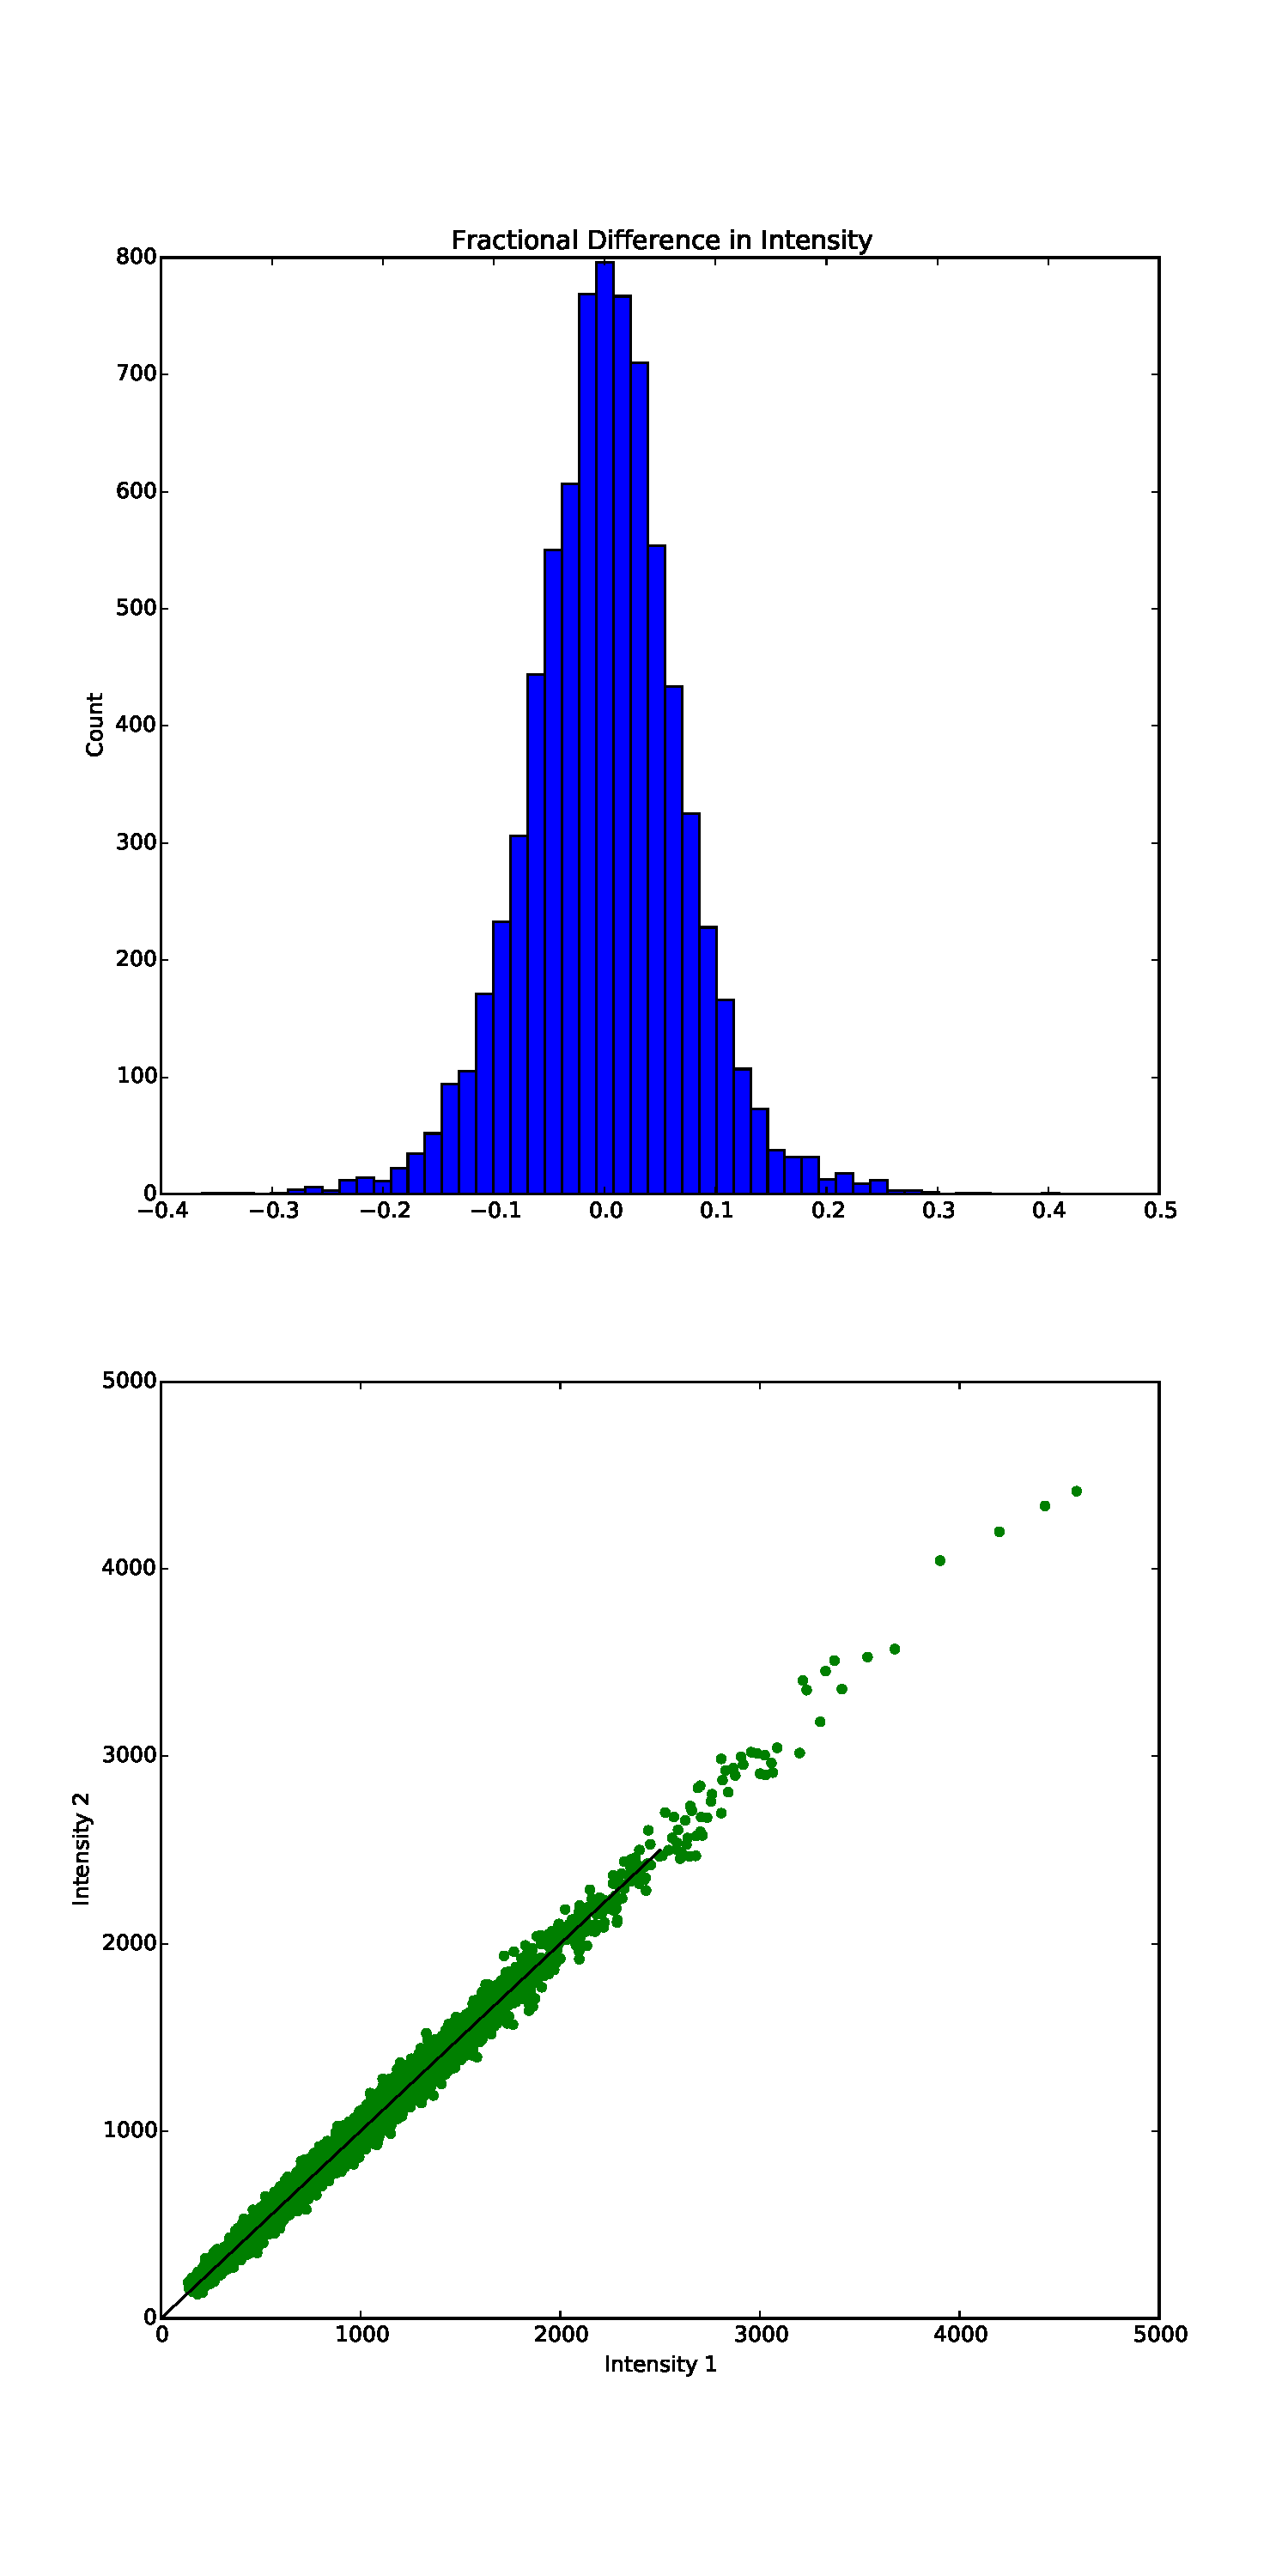
\includegraphics[height=0.9\textheight]{simtelerror1}
\caption{The fractional difference in total Image Intensity between the two simulations is shown in the graph above. A clear symmetric Gaussian is observed, with a mean of 0.00, and a standard deviation of 0.06. Below, the two intensities are plotted against one another. The distribution does not deviate significantly from the ideal 1:1 correspondence illustrated with the black line.}
\label{fig:simtelerror}
\end{center}
\end{figure} 

To assess the error in the LPD, a simulation of 2000 events was conducted with a fixed energy of 56TeV, and both Zenith and azimuth fixed to 0 degrees. The true distance to core was recorded from Sim\textunderscore telarray, and a graph was plotted of DC pixel intensity against core distance. As expected, a characteristic LPD is observed. Due to the application of a signal cut to the BDT candidates, we are only able to see the LPD at around $r_{core} \textgreater 35m$, at which point the LPD intensity crosses the threshold of 150 p.e. From here, there is a clear LPD continuing up to around 100m. Above roughly 100m, the LPD becomes dominated by highly random hadron fragmentation, and thus ceases to be coherent. The region 35-90m is considered, and if an exponential if fitted to the LPD, then the fractional deviation $\Delta_{TrueDC} = \frac{signal_{fit} - True_{DC count}}{signal_{fit}}$ can be found. Using the 68th centile of all absolute fractional deviations $\Delta_{TrueDC}$, we find that the LPD for $True_{DC}$ has an error of $\sigma_{TrueDC}=0.12$. Taking account of $\sigma_{STA}$, we deduce that the true associated error in the LPD is $\sigma_{TrueLPD} = \sqrt{(\sigma_{TrueDC}^{2} - \sigma_{STA}^{2})} = 0.11$. Thus we conclude that, in an ideal case, any LPD calculated from full shower images would always have a minimum error of 11\%. This is reasonably high, and can be partially explained by the random nature of atmospheric conditions, among other things.

The same exercise was repeated using the value of $DC_{Count}$ for the BDT candidate pixels in a full shower image, if the pixel had passed both the $DC_{Count}$ and $P_{signal}$ cuts. This provides a more reasonable estimate of the expected LPD error likely to be obtained experimentally, and includes the additional complication of having incorrectly identified pixels in the dataset. As before, the absolute fractional deviation of each pixel from the fit of the $True_{DC}$ LPD was found. Due to consistent underestimate of the $True_{DC}$ value using the simple $DC_{Count}$ method, the error was much larger, with $\sigma_{DCcount}=0.57$ and the $\sigma_{STA}$ being negligible in comparison. This representative error is extremely large, and will pose significant problems for event reconstruction.

\begin{figure}
\begin{center}
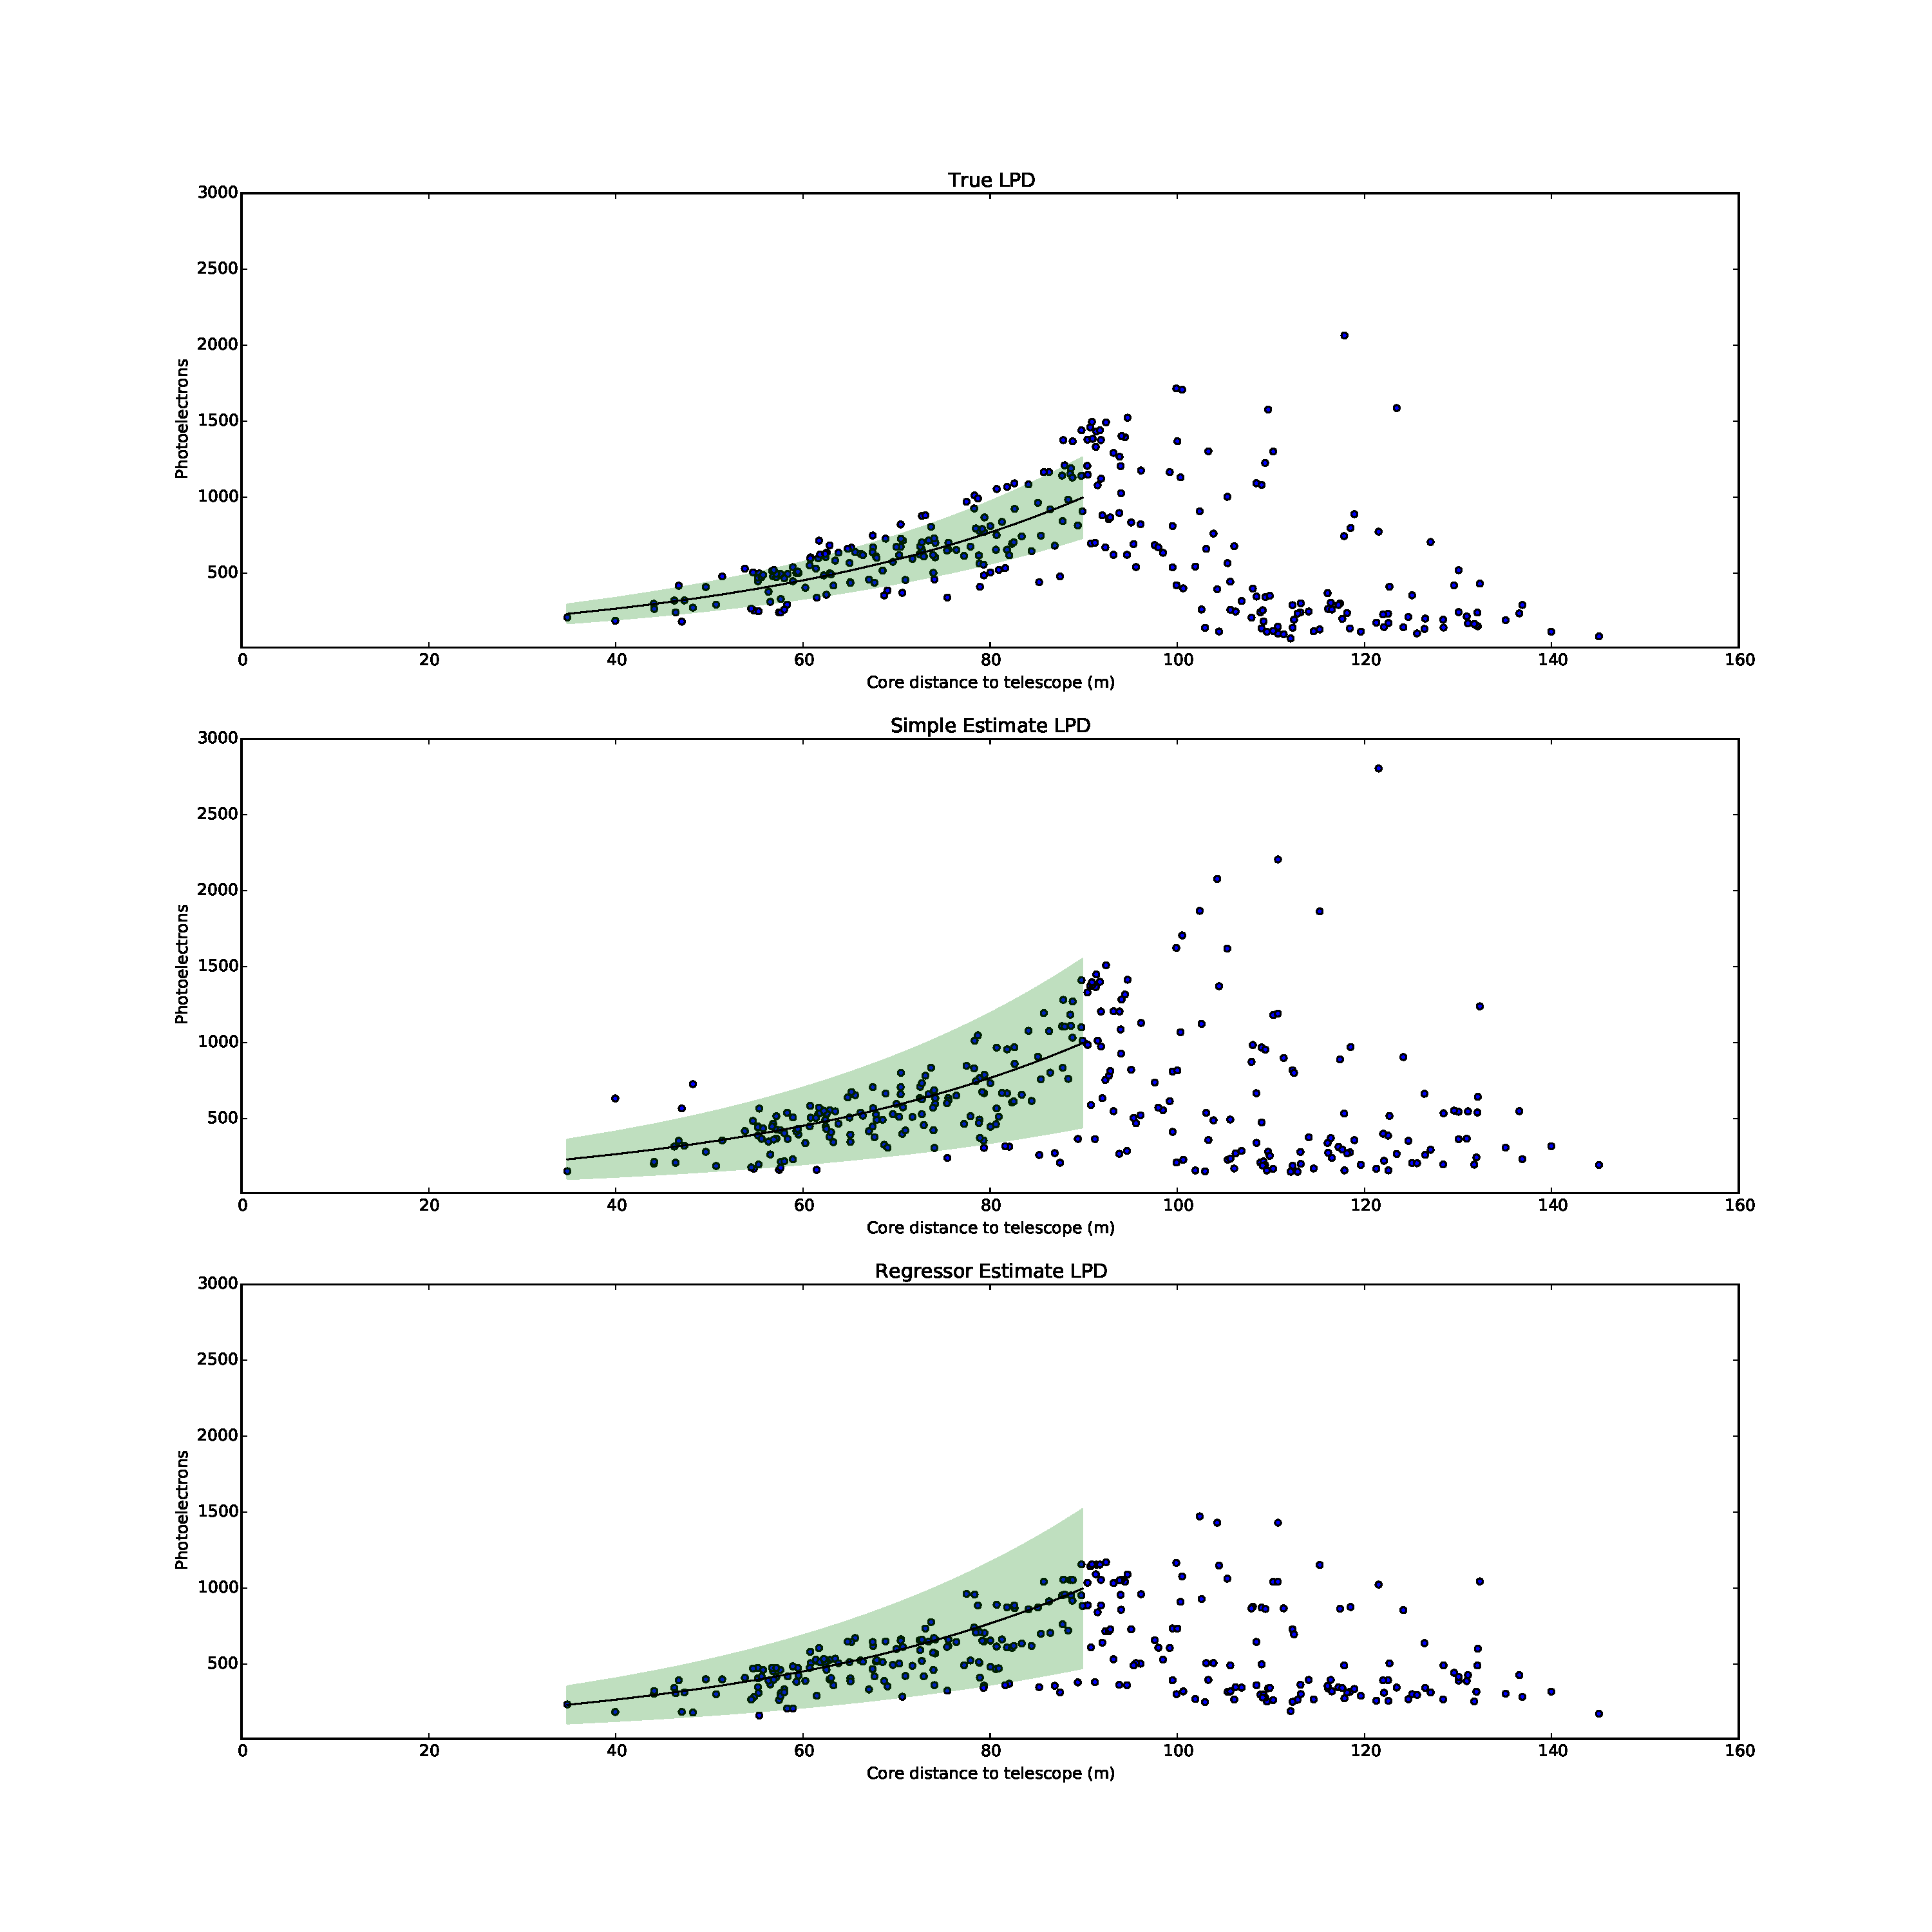
\includegraphics[width=\textwidth]{corsikalpd1}
\caption{The two LPDs shown above are estimates of HESS1 $True_{DC}$ calculated via $I_{tot}$, as well as for the maximum pixel $Intensity$. The two full-shower calculated LPDSs are shown underneath, with the simple guess $DC_{Count}$, and the regressor calculated $DC_{rgr}$. An exponential is fit to the $True_{DC}$ distribution, and the 68\% fractional deviation is shown in green. The same curve is shown on the two derived DC values, with the new fractional deviation being much greater.}
\label{fig:corsikalpd1}
\end{center}
\end{figure}

\begin{figure}
\begin{center}
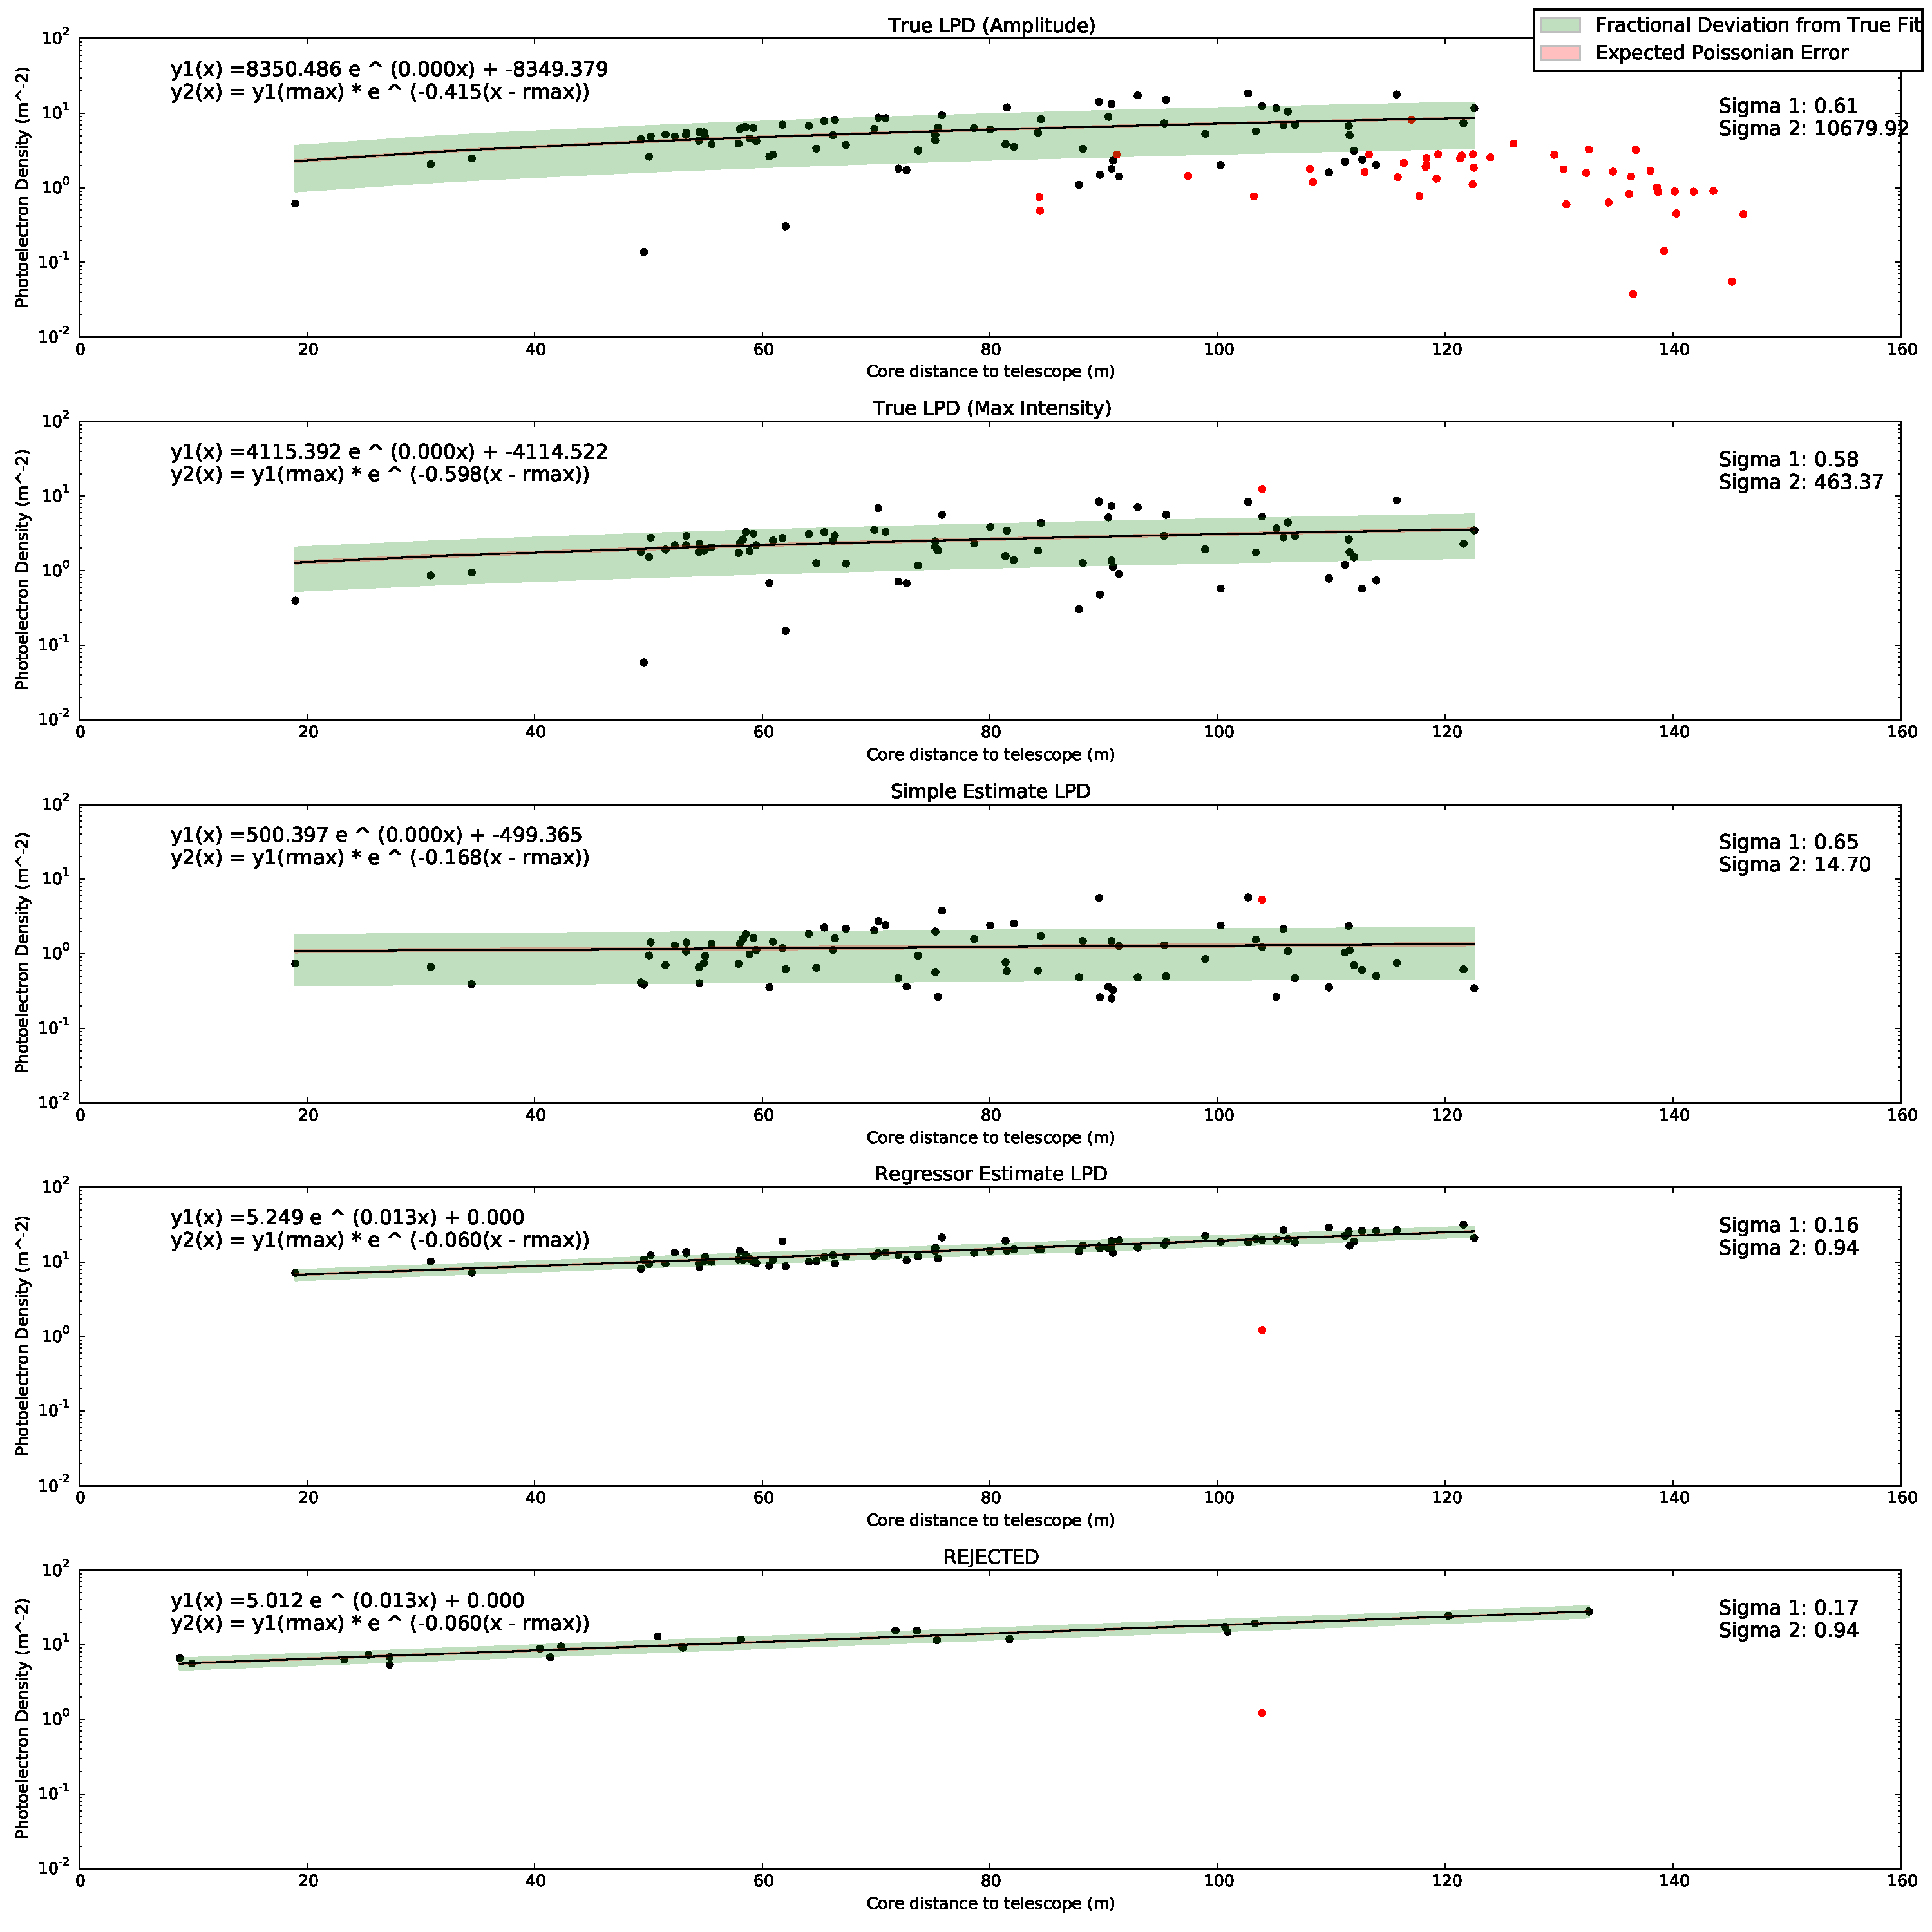
\includegraphics[width=\textwidth]{corsikalpd2}
\caption{The two LPDs shown above are estimates of HESS2 $True_{DC}$ calculated via $I_{tot}$, as well as for the maximum pixel $Intensity$. The two full-shower calculated LPDSs are shown underneath, with the simple guess $DC_{Count}$, and the regressor calculated $DC_{rgr}$. An exponential is fit to the $True_{DC}$ distribution, and the 68\% fractional deviation is shown in green. The same curve is shown on the two derived DC values, with the new fractional deviation being much greater.}
\label{fig:corsikalpd2}
\end{center}
\end{figure}

\subsection{Regression BDT for $DC_{Count}$}
In order to reduce the LPD error, an alternative method of calculating the DC signal was developed. Supervised machine learning was again used to solve the problem, by training a BDT Regressor. As with Classifiers, Regressors are initially trained using individual data entries. Instead of the true classes for the entries, regressors require the true value of a continuous variable. Once trained, the regressor can be used to predict a value of the variable for a given data entry. In this case, the Regressor is trained to estimate the quantity of DC light $True_{DC}$ for a given pixel. Once a DC pixel has been identified, the regressor is applied to it. The regressor returns the calculated value of $DC_{rgr}$, an alternative estimate of the DC signal. 

Accurate measurement of the value of $True_{DC}$ is hindered because the DC light can be split into multiple pixels. Instead of the brightest pixel intensity the total Image Amplitude in the EAS free image was used. However, for high altitude/zenith angles, the DC light may lie partially outside the telescope image. To account for this, a new training sample was simulated in CORSIKA with both zenith and azimuth angle fixed at 0. Despite intuitive expectation that regressor performance should worsen significantly when it was tested on the use 2000-event testing sample, the more accurate $True_{DC}$ values for the training more than compensated for this. 

The training set of data consisted of the true DC pixel in each full shower image. A regressor BDT was trained to extrapolate the DC signal, using the variables listed in Table \ref{tab:hess1regressor}. To account for the differing hardware, a separate regressor was trained, as before, for the CT5 camera. However, initial performance was poor, due to the size of the training dataset. Only one pixel per image was usable, leading to a small training dataset. Initial performance, as measured by deviation in \ref{fig:corsikalpd}, was initially poor. However, an expanded dataset of 5000 events greatly reduced the deviation from $True_{DC}$ values. The final BDT was trained with 1000 estimators and a max depth of 3. The Feature Importances for the HESS1 and HESS2 regressor are listed in Table \ref{tab:hess1regressor} and Table \ref{tab:hess2regressor} respectively. There is again a discrepancy in variable importance between the two BDTs.

\begin{table}[h!]
  \centering
  \caption{Relative Feature Importance in HESS-1 Regressor BDT training}
  \label{tab:hess1regressor}
  \begin{tabular}{ccc}
    \toprule
    Variable & Relative Importance\\
    \midrule
    $Q_{DC}$ & 0.17\\
    $DC_{Count}$ & 0.16\\
    Image Amplitude & 0.15\\
    $Intensity_{N.N.min}$ & 0.14\\
    $Intensity_{N.N.max}$ & 0.14\\
    $Intensity$ & 0.13\\
    $Mean_{N.N}$ & 0.11\\
    \bottomrule
  \end{tabular}
\end{table}

\begin{table}[h!]
  \centering
  \caption{Relative Feature Importance in HESS-2 Regressor BDT training}
  \label{tab:hess2regressor}
  \begin{tabular}{ccc}
    \toprule
    Variable & Relative Importance\\
    \midrule
    Image Amplitude & 0.20\\
    $Intensity_{N.N.min}$ & 0.15\\
    $Q_{DC}$ & 0.15\\
    $Mean_{N.N}$ & 0.14\\
    $DC_{Count}$ & 0.13\\
    $Intensity_{N.N.max}$ & 0.13\\
    $Intensity$ & 0.13\\
    \bottomrule
  \end{tabular}
\end{table} 

Repeating the comparison for the HESS1 regressor, we find for $\sigma_{rgrfit} = 0.35$, a significant improvement over $\sigma_{DCcount}$. Taking into account $\sigma_{STA}$, we find that ultimately $\sigma_{rgr}=0.34$, a fairly large value that nonetheless should be acceptable in 4-telescope events. The comparative performance is recorded in Table \ref{tab:lpderror}.

\begin{table}[h!]
  \centering
  \caption{Fractional error from fitted 56-TeV LPD distribution, accounting for $\sigma_{STA}$}
  \label{tab:lpderror}
  \begin{tabular}{ccc}
    \toprule
    & HESS1 & HESS2\\
    \midrule
    $\sigma_{TrueDC}$ & 0.13 & 0.18\\
    $\sigma_{DCcount}$ & 0.70 & 0.88\\
    $\sigma_{rgr}$ & 0.36 & 0.50\\ 
    \bottomrule
  \end{tabular}
\end{table} 

To get a more accurate estimate of the error, the testing set of 2000 events with varying azimuth/zenith was again considered. The fractional difference $\Delta = \frac{ candidate_{DC count} - True_{DC count}}{True_{DC count}}$ was binned in a histogram format, as shown in \ref{fig:dcdiff}. It was observed that the mean was 0.09 and the median was -0.08, meaning the distribution was partially skewed. If the absolute deviation from the $True_{DC}$ value is considered, then 68\% of pixels have a fractional deviation less than 0.33. Accounting for $\sigma_{STA}$, we find that the $sigma_{LPD}=\sigma_{rgr1}=0.32$, an improvement over the fixed 56Tev directly incident simulation.

For HESS2, the mean was 0.22 while the median was -0.09, leading to an even more skewed distribution. However the 68\% absolute fractional deviation was 0.29, and with $sigma_{STA}$, we find that $sigma_{LPD}=\sigma_{rgr2}=0.29$, slightly better than for HESS1. The improved performance can be explained by the matching energy distribution for the training and testing datasets. Higher-energy events have more background EAS light without consequently increased DC light, meaning the signal becomes harder to extract. The testing dataset has predominantly low-energy events, with reduced background.

We can parameterise the error by considering the energy and distance to the core for a selection of DC pixels. We find that, for a fixed energy...

56 and 26 teV comparison. Sigma is a function of E???


\begin{figure}
\begin{center}
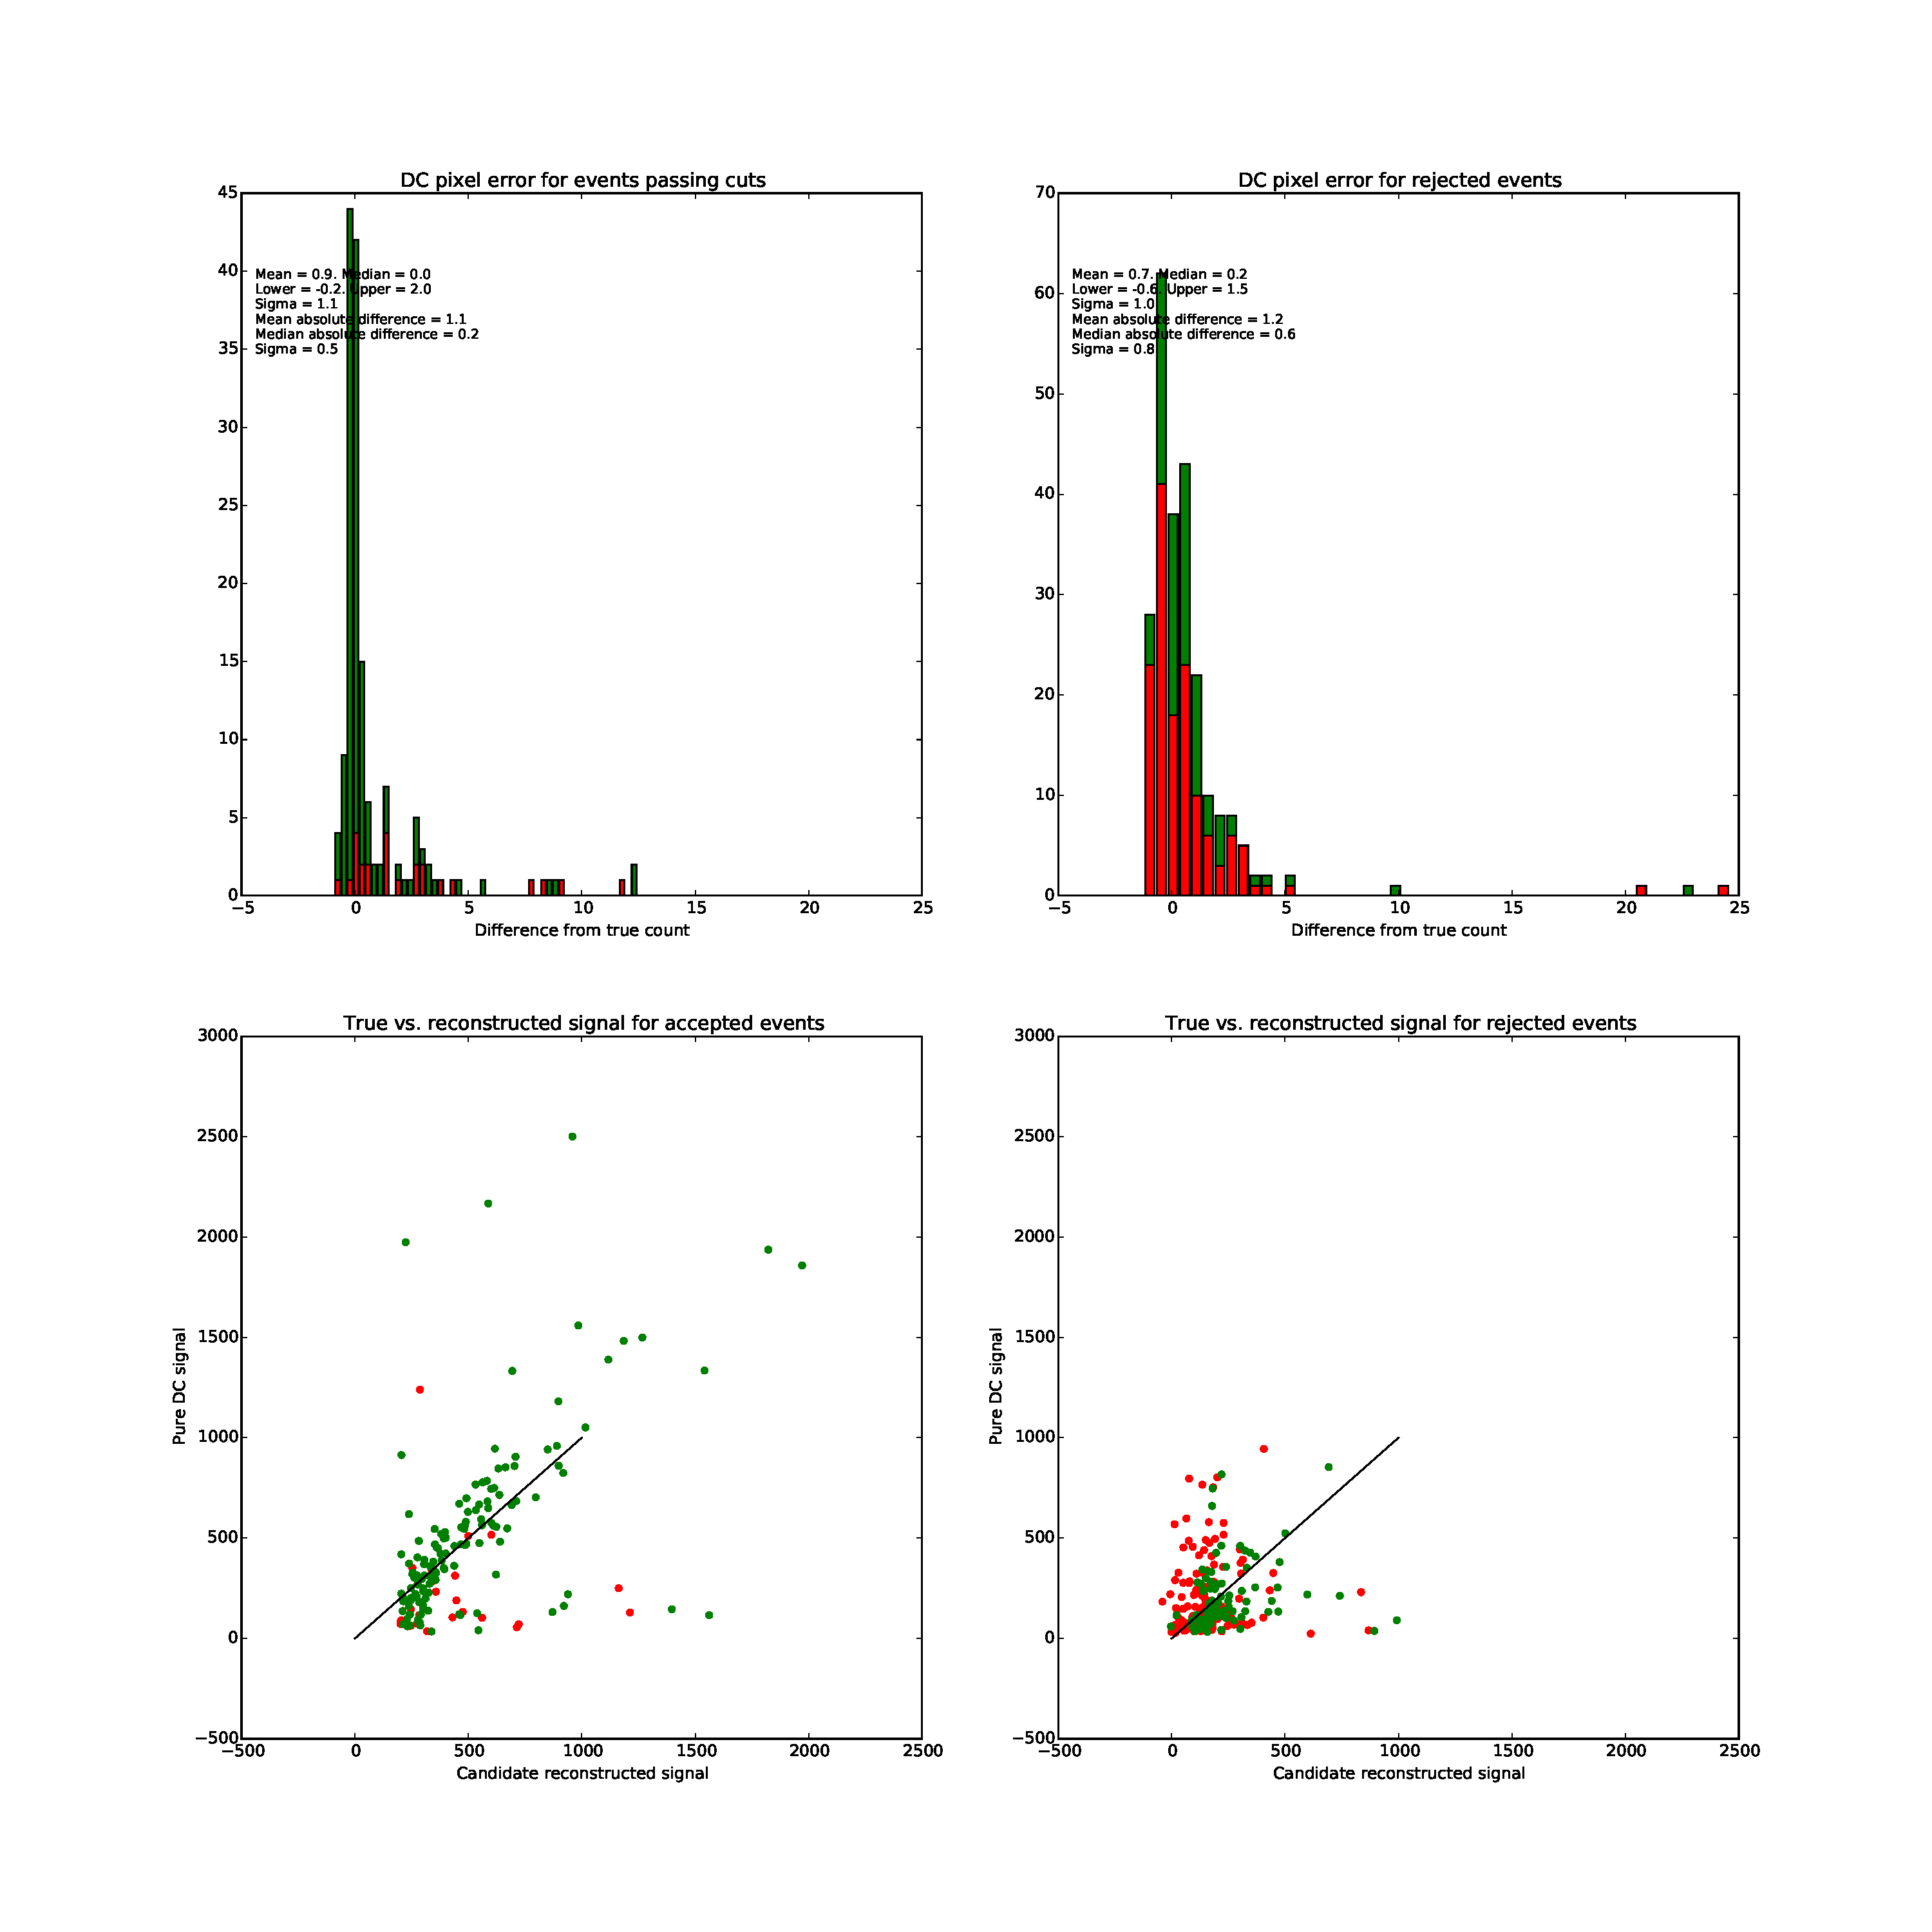
\includegraphics[width=\textwidth]{DCcounterrorhess1rgr}
\caption{The difference between true and reconstructed DC signal for events passing the cuts is shown in the top left. In the top right the same is shown for events which were rejected. The true DC signals for events which passed the cuts is plotted against the reconstructed signals in the lower left, and for rejected events in the lower right. As in \ref{fig:cutdistribution}, in all plots a green event is one in which the DC pixel has been correctly identified, while a red event is one that has been incorrectly identified.}
\label{fig:dcdiff}
\end{center}
\end{figure}

\section{HESS-type Event Reconstruction}
With a simulation of the HESS Cherenkov 5-Telescope Array we can verify the effectiveness of the technique. 
\subsection{First Interaction and Energy Saturation}
The mean first interaction height for all Cherenkov Emitting Cosmic Rays in the atmosphere is 40km, and neglecting variations in atmospheric density profiles around the Earth, this can be considered independent of experimental array. However, the multiplicity of event is determined by equipment efficiencies, altitude and telescope layout. When the HESS layout is simulated, we find that the 4 telescope events have a mean height of $h \approx 23 \pm 5$ km, as shown in \ref{fig:Hessheight}.

\begin{figure}
\begin{center}
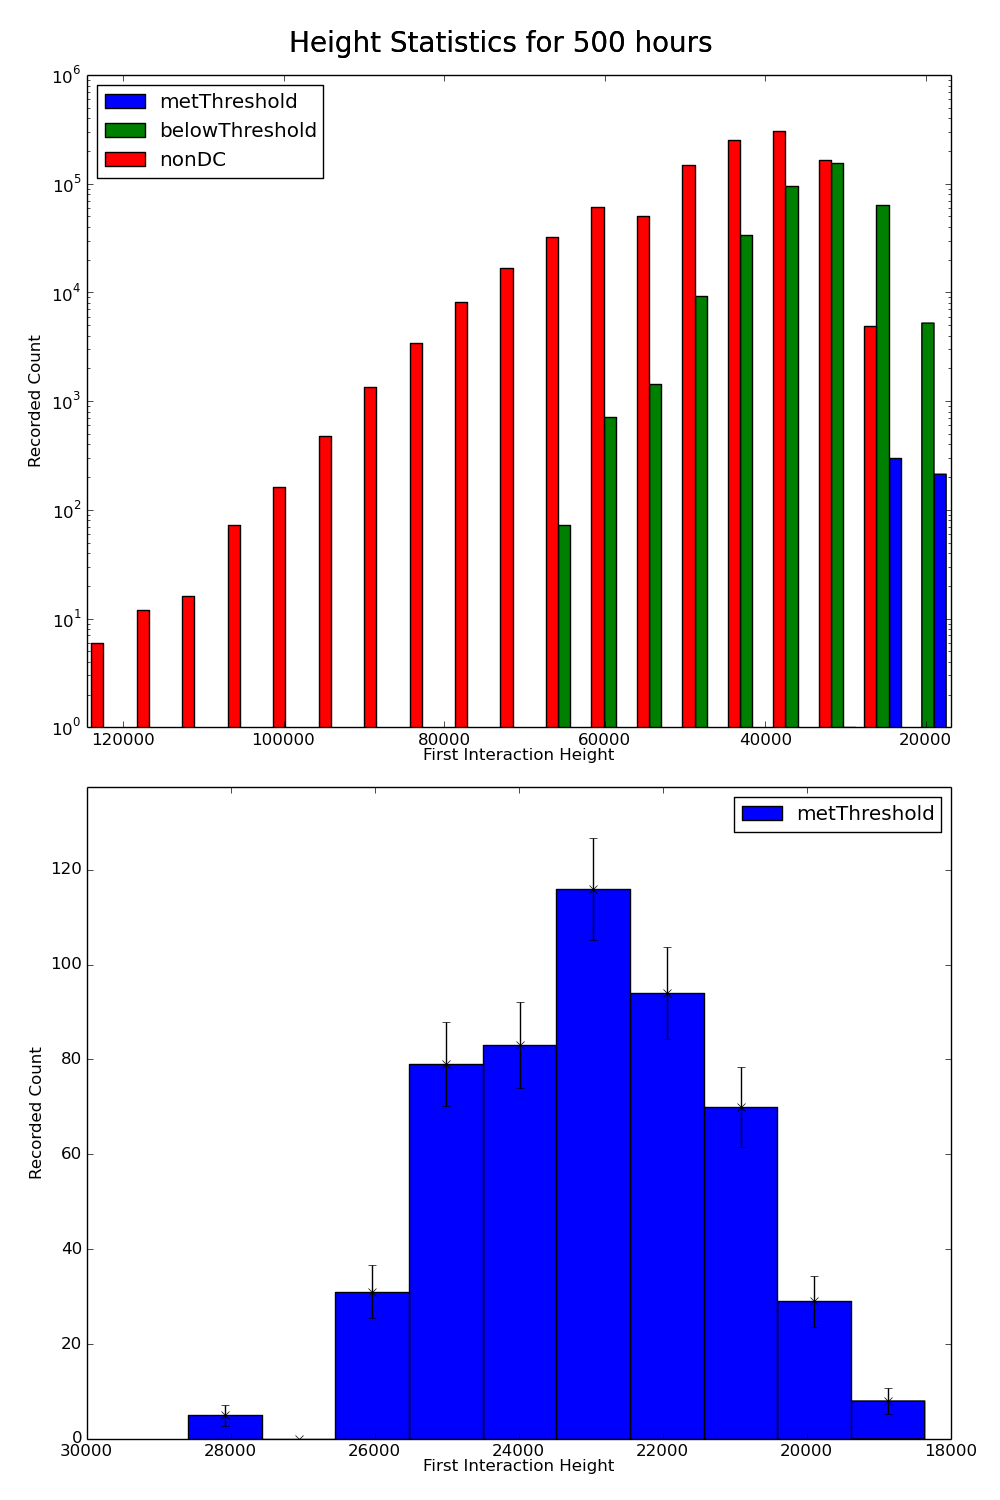
\includegraphics[height=0.9\textheight]{hessheight}
\caption{The mean first interaction height for all Cherenkov Events is 40km???. The mean first interaction height for 4 telescope events in the HESS array is 23km}
\label{fig:Hessheight}
\end{center}
\end{figure}

\subsection{Extended Air Shower Background}
A typical HESS image is shown in \ref{fig:hess}, with the DC pixel visible. For HESS cameras, the Extended Air Shower (EAS) produced after the first interaction of the Cosmic Ray overlaps the DC pixel and thus provides background in the LDF. As the Energy of the Cosmic Ray increases, the EAS speads over a larger angular area, and at smaller radii, the EAS-DC-shower direction axis contracts, leading to more overlap. Thus the background in the DC pixel increases with decreasing radius and increasing Energy. In addition, we have a fixed night sky background with 7 photons $m^{-2}$. We thus parameterise the background with \[ \rho_{bkg}  = 7 + 5E\]. The modeled background LPD is shown as part of REF. It begins to dominate above roughly 1 TeV per Nucleon, particularly in the case of smaller radii. 

\begin{figure}
\begin{center}
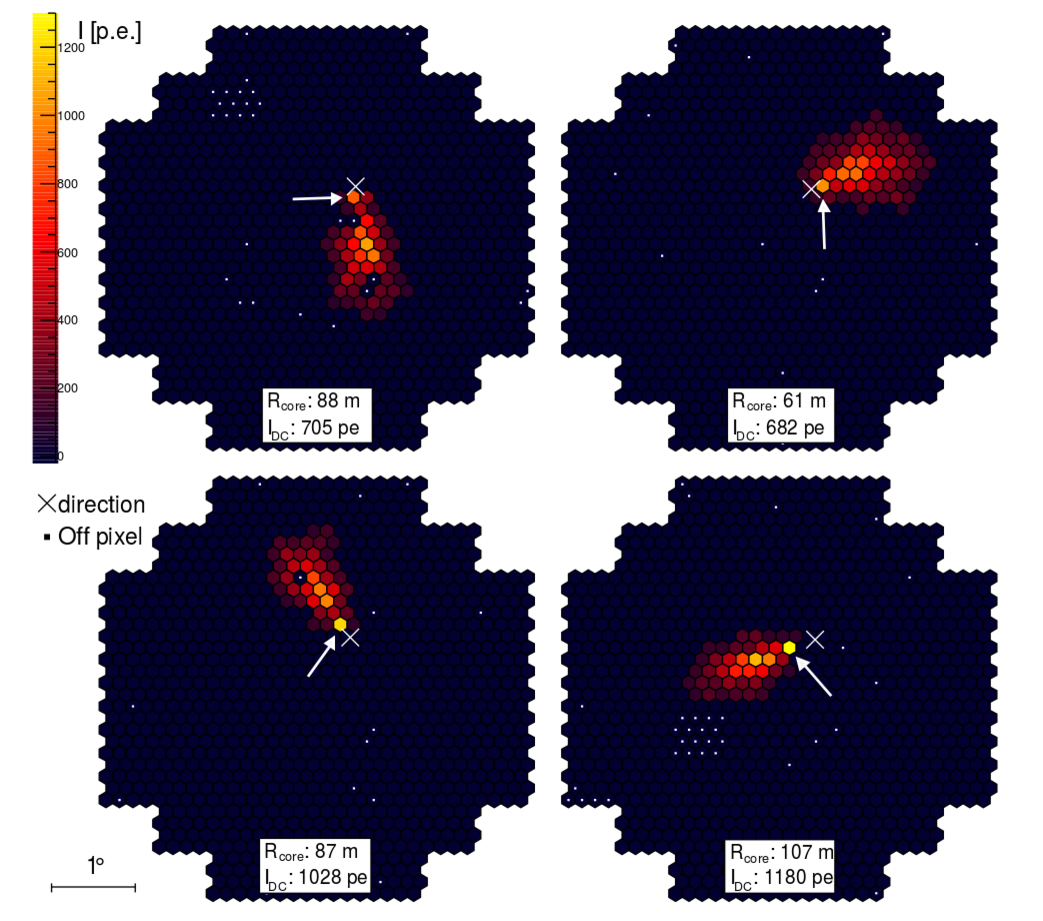
\includegraphics[width=0.9\textwidth]{hess}
\caption{A 4-camera HESS event. The shower direction is marked with a white cross, and the DC pixel is indicated with a white arrow. The shower axis passes through the shower direction, the DC pixel, and the center of the Extensive Air Shower region lying beyond the DC pixel.}
\label{fig:hess}
\end{center}
\end{figure}

\subsection{Reconstructed Charge Resolution}
In the preliminary HESS simulation, it was found that the 4 telescope event reconstruction had a charge resolution of $\sigma_{Z} = 1.4$. However, requiring that the BDT signal probability satisfied $P > 0.81$ removed $75 \%$ of events, while reducing the Charge resolution to $\sigma_{Z} = 0.9$ . With this cut, core position resolution was $d \approx 1.4 m $. For 5 telescope events, it was found that the charge resolution was also $\sigma_{Z} = 1.4$. However, requiring that the signal probability satisfied $P > 0.05$ removed $53 \%$ of events, including all wrongly reconstructed ones. This placed an upper limit on the charge resolution of $\sigma_{Z} < 0.35$ . With this cut, core position resolution was $d \approx 0.8 m $.

However, the simulated number of hours for the data was 1200? hours, and comparisons with HESS data show just 12 4-telescope events rather than 600. Thus, although the technique is valid and effective for HESS, the count rate will limit the potential to conduct any statistical analysis from this experiment.

\section{Optimised Telescope Array}
NO Background!!!!!
\subsection{Count Rates}

In order to improve the count rate of high-multiplicity events, we can consider a 3x3 array of Cherenkov Telescopes, which we want to use for identifying Cosmic Ray Elements accurately. In \ref{fig:optmiselayout} we see that the \textquoteleft High Multiplicity Count Rate' of events observed by 4 or more telescopes falls with increasing grid separation. We can clearly see that the optimum grid spacing will likely lie in the 20-50m region to provide a reasonable count rate. Competing with this effect is the reliance of LDF reconstruction on sampling the entire lateral distribution. Thus the reconstruction quality will decrease as Grid Width decreases. Further study of $\sigma_{Z}$ in this region is required to determine the optimum layout (not necessarily be a grid) for event reconstruction. 

\begin{figure}
\begin{center}
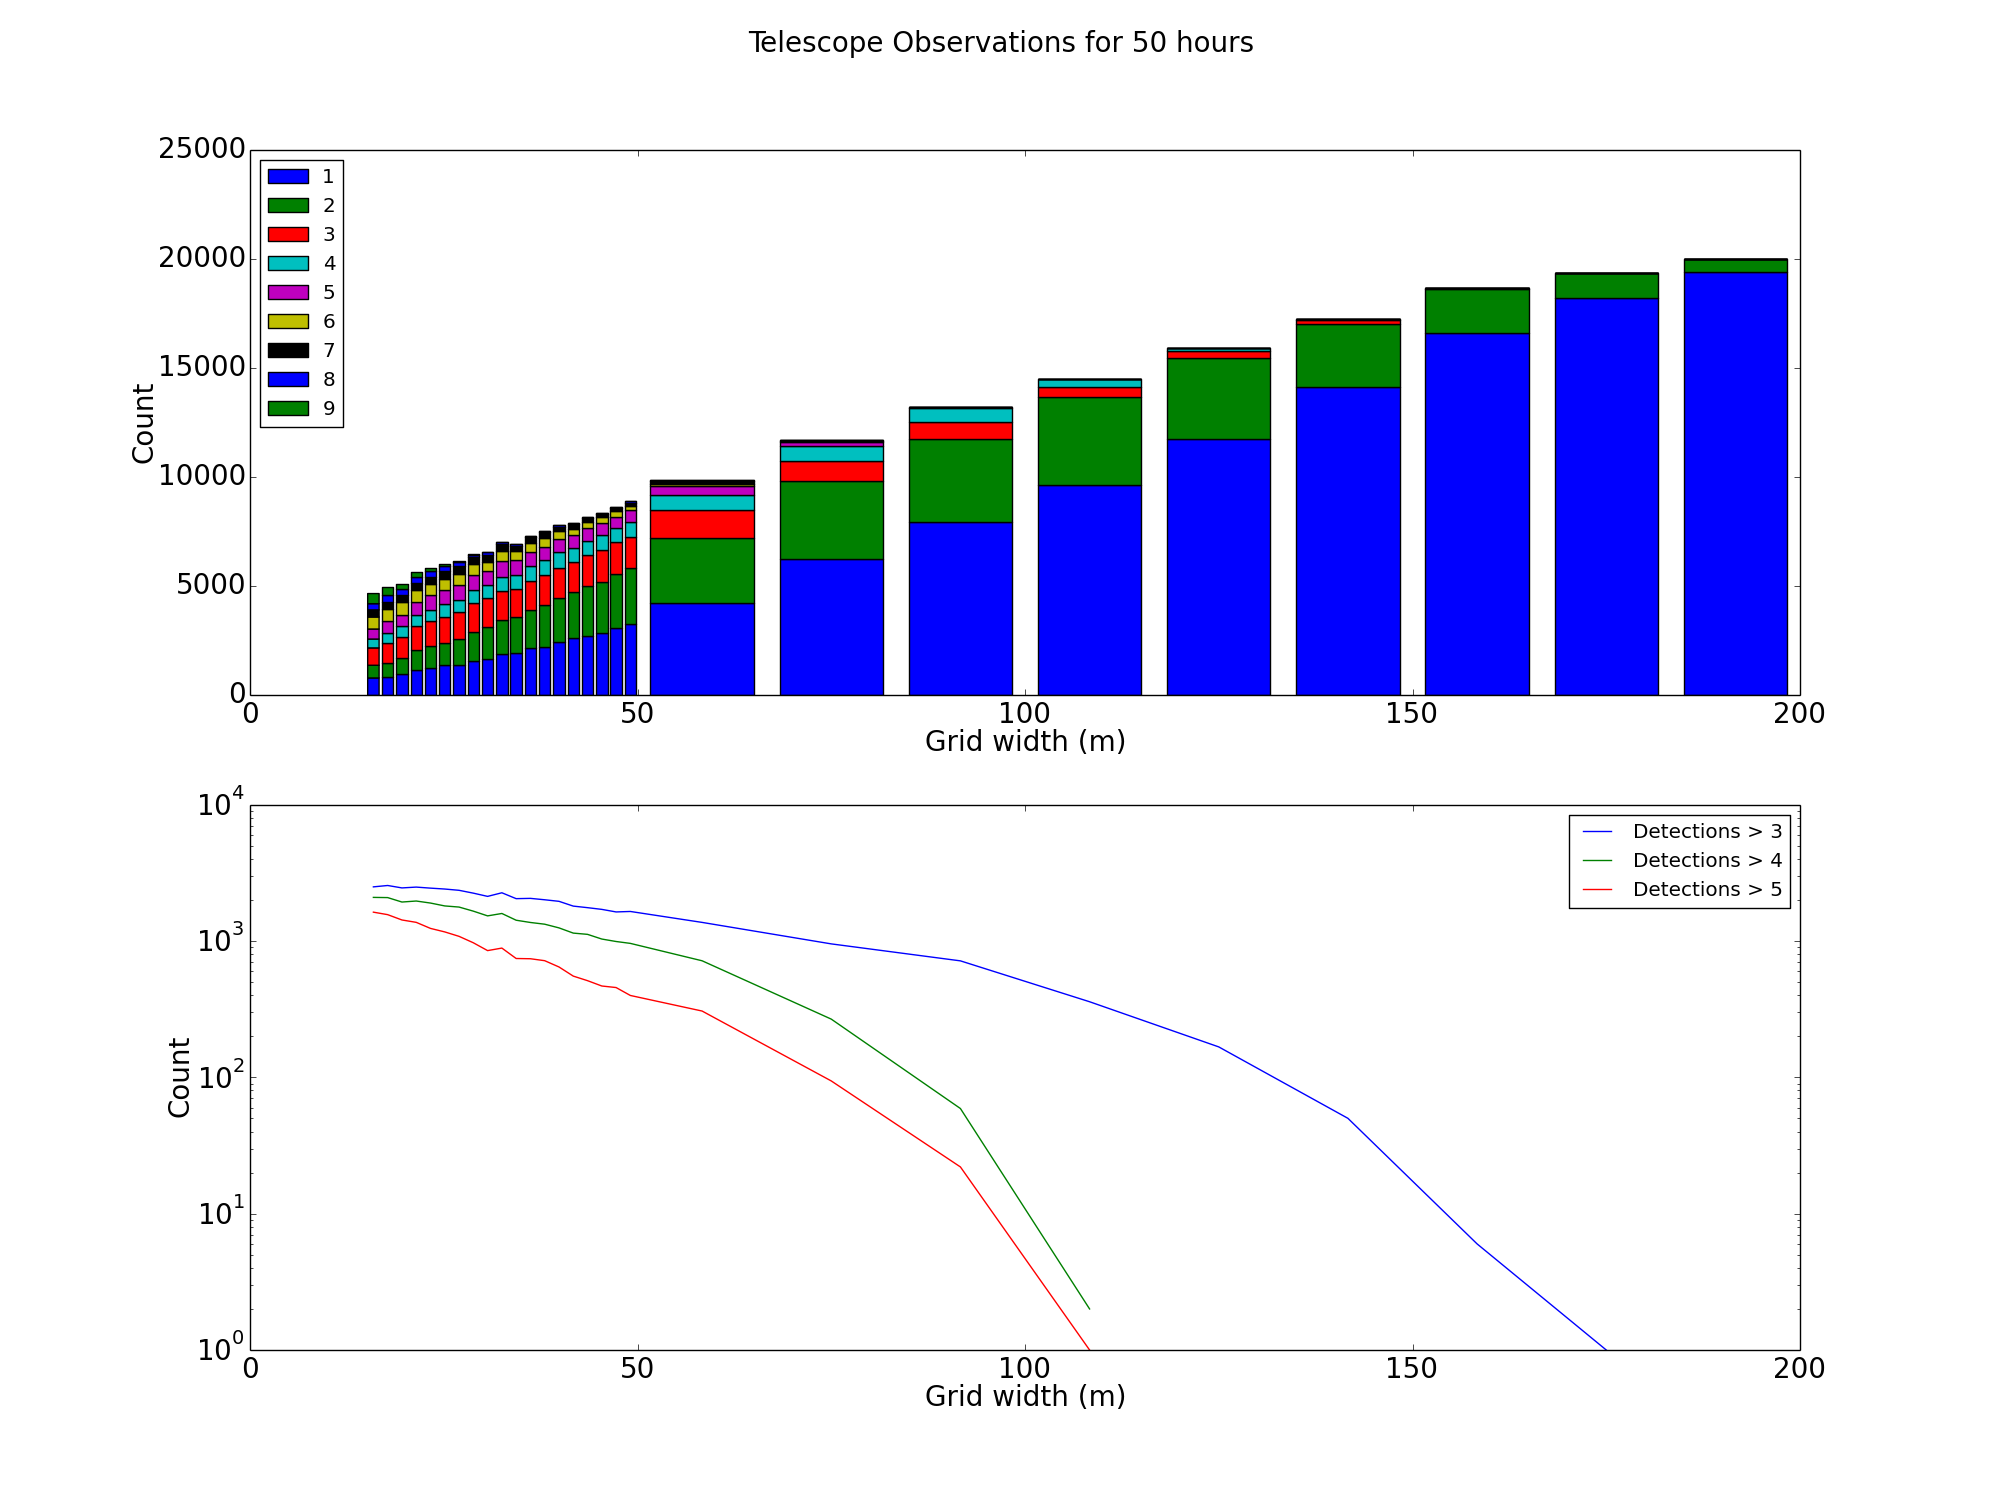
\includegraphics[width=0.9\textwidth]{optimiselayout}
\caption{A simulation of 50 hours of run time for various grid spacing for a 3x3 telescope array. Although raw count rate increases with increasing grid width, the \textquoteleft good count' rate of events observed by sufficient telescopes falls rapidly with increasing grid width}
\label{fig:optmiselayout}
\end{center}
\end{figure}

\subsection{Saturation Region Energies}

\subsection{High Speed Telescopes}
By definition, the EAS shower will arrive on the ground shortly before the DC light. There are currently several high-speed Cherenkov telescopes capable of distinguishing between these, allowing a background-free LDF to be fitted. Additional study of alternative energy regimes and layouts will also be considered for the case of a high-speed imaging telescope array. 

\section{Conclusion}
Preliminary results suggest that the LDF reconstruction technique will significantly improve charge reconstruction, to a level sufficient for cosmic ray abundance studies. However, reliance on high-multiplicity events means that although applicable to current experiments such as HESS, a new optimised telescope array would be required for a statistical analysis. Such an array may have a grid spacing of 20-50m, although further study is needed to determine the ideal layout.
\bibliographystyle{unsrt}
\bibliography{report}
\end{document}